%\documentclass[10pt]{article} % Reduced font size slightly to help with page count
\documentclass[11pt]{article}
\usepackage{times}
\usepackage{enumitem}
\usepackage{mathptmx} % Times New Roman font
\usepackage{booktabs}
\usepackage{multirow}
\usepackage{array}
\usepackage{float}
\usepackage{longtable} % For potentially very long tables
\usepackage{cite}
\usepackage{graphicx}
\usepackage{url}
\usepackage[numbers]{natbib}
\usepackage{hyperref}
\hypersetup{
    colorlinks=true,
    linkcolor=blue,
    filecolor=magenta,
    urlcolor=cyan,
    citecolor=blue, % Make citations visible
}

\usepackage{tikz}
\usepackage{pgfplots}
\pgfplotsset{compat=1.17}
\usepackage{pgf-pie}
\usepgfplotslibrary{colorbrewer}
\pgfplotsset{cycle list/Set1-5}
\usepackage{graphicx}

\usepackage{pgfplots}
\pgfplotsset{compat=1.18} % Or any recent version you have
\usepackage{float}

\usepackage{geometry}
\usepackage{amssymb}
\usepackage{tcolorbox}
\usepackage{xcolor}
\usepackage{tabularx}
\usepackage{amsmath} % For potential equations
\usepackage{caption} % For better caption control
\usepackage{setspace} % To potentially adjust line spacing if needed for length
\usepackage[utf8]{inputenc} % Ensure UTF-8 encoding
\usepackage{fontenc} % Use T1 font encoding

\usepackage{ragged2e}
\usepackage{hyphenat}
\newcolumntype{P}[1]{>{\RaggedRight}p{#1\linewidth}}

\usepackage{pgfplots}
\usepackage{pgf-pie}
\pgfplotsset{compat=1.18}

\usepgfplotslibrary{colorbrewer}
\pgfplotsset{cycle list/Set1-5}

\usepgfplotslibrary{colorbrewer}
\pgfplotsset{cycle list/Set1-5}

% Adjust geometry for potentially more content per page
\geometry{a4paper, top=2.5cm, bottom=2.5cm, left=2cm, right=2cm, headheight=13.6pt}
\usepackage{fancyhdr}
\usepackage{pgf-pie}
% Define checkmark and crossmark symbols (using pifont or amssymb)
\usepackage{pifont} % Or use \usepackage{amssymb}
\newcommand{\cmark}{\ding{51}}%
\newcommand{\xmark}{\ding{55}}%

% Potentially adjust line spacing to manage length
% \setstretch{1.1} % Slightly increase line spacing

\title{AI-Powered Audio-Visual Intruder Detection in Smart Homes: A Systematic Literature Review}

\date{} % Remove date


\begin{document}

\begin{center}
    % Ensure the image path is correct relative to the.tex file location
    % If 'images' is a subfolder:
    \includegraphics[width=0.5\textwidth]{images/TUTlogo.png}
    % If the logo is in the same folder:
    % \includegraphics[width=0.25\textwidth]{TUTlogo.png}
\end{center}

\begin{center}
    \vspace{0.2cm}
    {\Large{Faculty of Information and Communication Technology}} \\[0.1cm]
    {\large{Department of Computer Systems Engineering}} \\
\end{center}

\begin{center}
    \vspace{0.5cm}
    {\huge{AI-Powered Audio-Visual Intruder Detection in Smart Homes: A Systematic Literature Review}} \\
    \vspace{1cm} % Add more space before authors
\end{center}

\begin{center}
    \begin{minipage}{1\textwidth}
        \centering
        \textbf{Desmond Makhubela\textsuperscript{1,*}}, 
        \textbf{Munguakonkwa Emmanuel Migabo\textsuperscript{2,*}(Supervisor)}, 
        \textbf{Oluwasogo Moses Olaifa\textsuperscript{1,*}}, 
        \textbf{Chunling Du\textsuperscript{1,*}}

        \vspace{0.5cm}

        \centering
        \textsuperscript{1} Department of Computer Systems Engineering, Tshwane University of Technology, Pretoria, South Africa \\
        \textsuperscript{2} Department of Electrical Engineering, Tshwane University of Technology, Pretoria, South Africa \\
        \vspace{0.3cm} % Add space before correspondence
        \textsuperscript{*} Correspondence: 214396874@tut4life.ac.za(D.M), migabome@tut.ac.za (M.E.M.); duc@tut.ac.za (C.D.); olaifamo@tut.ac.za (O.M.O.)\\
    \end{minipage}
\end{center}

\vspace{1cm} % Add space before abstract/introduction


\begin{abstract}
This systematic literature review explores the application of AI-powered audio-visual systems for intruder detection in smart homes. Conventional systems, which rely on isolated motion sensors or CCTV, are limited by high false alarm rates and reduced reliability. Recent advancements integrate multimodal data fusion—combining audio and visual inputs—processed through artificial intelligence models such as convolutional neural networks (CNNs), transformers, and hybrid fusion architectures. These approaches enhance detection accuracy, contextual awareness, and robustness. This review, conducted using a PRISMA-based methodology, synthesizes current strategies, compares data fusion techniques, and evaluates the trade-offs between hardware platforms such as Raspberry Pi and GPU-based systems designed for real-time performance. Emerging trends, including privacy-preserving edge computing, are also examined. The findings identify key challenges and offer recommendations to guide future research toward the development of low-cost, accurate, and user-friendly smart home security solutions
\end{abstract}

\newpage
\begin{center}
    \vspace{0.5cm}
    \textbf{Keywords:} Smart Home Security, Audio-Visual Analysis, Intruder Detection, Edge AI, Multimodal Fusion, Privacy-Preserving Techniques
\end{center}

\section{Introduction}
\subsection{Context and Importance of the Topic}
Ensuring residential security is a global concern, irrespective of geographic or socio-economic contexts. Protecting ourselves from break-ins, unwanted visitors, and other security issues is essential. These problems can threaten not only our belongings but also our personal safety. Over the years, new technologies have been developed to improve home security. Many traditional home security systems use basic tools like Passive Infrared (PIR) motion detectors and Closed-Circuit Television (CCTV) cameras. However, these older systems have some problems. A major issue is that they often cause false alarms. This happens when the alarms go off without a real danger. False alarms can be triggered by harmless things such as pets moving, changes in shadows, objects blowing in the wind, or typical household noises \cite{oduah_et_al_2025}. 
When alarms go off repeatedly for no real reason, people might start to ignore them, a phenomenon termed 'alarm fatigue' may occur. It leads to people not reacting to the security system, even when there is a real threat. Over time, this can make people feel the security system is not very effective or useful \cite{eutizi_benedetto_2021}.
\\
\\
Although there are advancements in sensor technology, distinguishing real threats from everyday activities in homes remains difficult. This difficulty exists because sensors have their own limits and homes differ in lighting, sounds, and activities \cite{sudharsanan_et_al_2024}, \cite{harini_et_al_2024}. Frequent false alarms can cause people to lose faith in their security systems. This is more than just a bother; it's a significant problem. If people don't trust their security systems, they might turn them off or ignore them, making their homes unsafe. Therefore, it's essential to improve security systems so they can effectively distinguish between true threats and harmless activities. These improvements are not only about better technology but also about maintaining people's trust to ensure the systems protect as they should. Combining different sensors, like those for sound and video, with smart software can help address these issues. This approach offers better information to help determine if a threat is genuine \cite{abdullah_noah_}, \cite{malar_dineshkumar_2024}.

\subsection{Current State of Knowledge}
Traditional security methods have shown clear shortcomings—something the research world can no longer ignore. In response, experts are turning to the cutting edge of technology: Artificial Intelligence and Machine Learning. These powerful tools are opening the door to smarter, more adaptive, and far more dependable home security systems than ever before. \cite{ali_et_al_2023, malar_dineshkumar_2024}. AI-based systems process sensory input more adaptively, distinguishing real threats from background activities. By using advanced algorithms to sift through data from devices like high-resolution cameras and sensitive microphones, they can spot danger with impressive accuracy while ignoring false alarms. However, this leap in intelligence doesn’t come without a cost. The hardware needed, such as GPU-powered processors and cutting-edge sensors, can be extremely expensive, placing them out of reach for many homeowners. On top of that, the setup process can be intimidating. Installing, configuring, and maintaining these complex systems demands not just money, but technical knowledge and a lot of energy. As a result, despite their advantages, they often remain less practical than the more straightforward, budget-friendly options they aim to replace. \cite{tomar_et_al_2022}. Consequently, the market bifurcates into high-end intelligent systems and affordable, yet often less reliable, alternatives.
\\
\\
Although sensor technology has advanced significantly, researchers are exploring a wide range of technical solutions to bridge this gap. In the realm of visual analysis, Convolutional Neural Networks (CNNs) have emerged as a foundational tool. These models are widely used to detect human presence, interpret specific behaviors, and flag unusual activity within video feeds, making them central to many AI-driven surveillance systems. \cite{dinama_et_al_2019, malar_dineshkumar_2024}. Related visual processing tasks relevant to security include human identification within surveillance footage \cite{jin_et_al_}, classification of human activities to distinguish normal behavior from suspicious actions \cite{zaidi_jagadeesh_2017, stephens_bors_}, and detecting actions even in challenging crowded scenes \cite{guo_2010}. Image processing techniques, such as those based on Local Binary Pattern histograms, are also explored for surveillance and intrusion detection \cite{archana_et_al_2022, sivakumar_2018}. For audio analysis, techniques often involve transforming sound signals into visual representations like spectrograms (time-frequency plots) which can then be analyzed, often using CNNs as well, to identify specific sound events indicative of intrusion, such as breaking glass, forced entry noises, or even specific human speech patterns \cite{harini_et_al_2024, kumar_et_al_}. Foundational work in audio analysis for surveillance applications laid the groundwork for these methods \cite{radhakrishnan_divakaran_smaragdis_2005}. More advanced techniques might involve analyzing acoustic unit occurrence patterns \cite{kumar_et_al_} or using layered symbolic sequence representations \cite{lai_burred}. Some research even explores the link between audio cues and human motion \cite{ofli_et_al_}.

The core idea gaining traction is the synergistic use of both modalities through sensor fusion. By combining information from audio and visual streams, systems can potentially achieve a higher level of certainty and robustness than systems relying on a single sensor type \cite{abdullah_noah_}. For instance, the sound of breaking glass combined with the visual detection of motion near a window provides much stronger evidence of an intrusion than either cue alone. This multimodal approach aims to leverage the complementary strengths of audio and visual data while mitigating their individual weaknesses (e.g., visual systems impaired by poor lighting, audio systems affected by background noise). A significant research thrust exists in bridging the gap between the high accuracy potential of advanced AI models and the practical constraints of cost and computational resources in consumer-grade smart home devices.
\\
\\
The exploration of platforms like Raspberry Pi and Arduino \cite{tomar_et_al_2022, nadaf_et_al_2020, owoeye_et_al_2025} reflects this effort. These platforms offer affordability and accessibility but possess limited computational power compared to high-end servers or workstations. Consequently, achieving robust AI performance on such resource-constrained hardware necessitates research into model optimization techniques (e.g., quantization, pruning) or the development of inherently lightweight yet effective AI architectures. This trade-off between performance, cost, and real-time processing capability on edge devices is a defining characteristic of current research in practical smart home security systems. Furthermore, recent advancements in AI, such as Transformer models and attention mechanisms originally developed for natural language processing, are being adapted for audio-visual analysis, potentially offering new ways to model temporal dependencies and cross-modal relationships. Integrating findings from these cutting-edge research areas is crucial for understanding the future trajectory of the field \cite{chopra_et_al_2023}.

\subsection{Rationale for the Systematic Literature Review}
Although research on intelligent home security is expanding rapidly, there’s still a clear need for a focused review on how AI-driven audio-visual analysis is being applied. Most existing systems rely heavily on a single type of input—either sound or visuals or use AI in a limited and often surface-level capacity. This Systematic Literature Review (SLR) aims to bring together and critically assess the latest innovations that combine auditory and visual data, processed through advanced AI algorithms, to create more robust intruder detection systems for residential environments. The primary aim is to investigate how this multimodal approach can address key limitations, such as frequent false alarms in traditional setups and environmental weaknesses in single-modality AI systems. The review places particular focus on striking the right balance between technical performance (like accuracy and dependability) and practical concerns (such as cost, complexity, and energy use). Of special interest is the potential to pair low-cost hardware with sophisticated AI to develop smarter yet more accessible home security solutions.
\\
\\
By examining the effectiveness of various AI-based fusion strategies, identifying common hurdles, and spotting emerging trends, this review intends to offer a comprehensive snapshot of where the field currently stands. Ultimately, it aims to steer future research and innovation toward building more reliable, affordable, and user-friendly smart security systems for everyday homeowners. \cite{abdullah_noah_}.

\subsection{Objectives and Research Questions}
This systematic literature review is guided by the following specific objectives and research questions (RQs):
\subsubsection{Research Objectives}
This study aims to find and understand the common audio-visual techniques, such as feature extraction, AI models, and fusion methods, used in smart home intruder detection systems. It also looks at how well AI algorithms improve accuracy, reliability, and reduce false alarms compared to traditional or single-modality systems. The review checks out the types of audio and video devices, processing platforms, such as affordable ones like Raspberry Pi, and system designs used for collecting and processing data. It also explores the main technical, practical, and ethical challenges in building and using AI-powered audio-visual intruder detection systems. Lastly, it examines new trends, future research paths, and possible tech advancements in smart audio-visual home security.
\subsubsection{Research Questions}
\begin{enumerate}
    \item What are the common audio-visual analysis techniques (including feature extraction, AI models, and fusion strategies) used in smart home intruder detection systems?
    \item How effective are AI algorithms in improving the accuracy, reliability, and false alarm reduction capabilities of these systems compared to traditional or single-modality approaches?
    \item What types of audio and video acquisition devices, processing platforms (including low-cost options like Raspberry Pi), and system architectures are commonly utilized for data acquisition and processing in these systems, and what are the emerging trends and future research directions shaping their development?
    \item What are the key challenges and limitations (technical, practical, ethical) currently faced in the development and deployment of AI-powered audio-visual intruder detection systems?
\end{enumerate}


\subsection{Contributions}

This systematic literature review aims to make several contributions to the field of smart home security, which are summarized in Table~\ref{tab:contributions} and elaborated below.

\begin{table}[h]
\centering
\caption{Summary of Key Contributions}
\label{tab:contributions}
\begin{tabular}{|p{3cm}|p{10cm}|}
\hline
\textbf{Type} & \textbf{Contribution Summary} \\ \hline
Theoretical & Comprehensive synthesis of AI approaches using audio and visual data for home intruder detection. \\ \hline
Theoretical & Structured comparative analysis of detection methods, data types, hardware platforms, and target environments. \\ \hline
Practical & Examination of practical trade-offs in using cost-effective hardware like Raspberry Pi with advanced algorithms. \\ \hline
Practical & Identification of research gaps including dataset standardization, real-world robustness, scalability, and privacy. \\ \hline
Practical & Recommendations for future research directions focused on affordable, reliable, and ethical home security solutions. \\ \hline
\end{tabular}
\end{table}

\vspace{1em}

\noindent The contributions can be grouped into theoretical and practical insights as follows:

\paragraph{Theoretical Contributions:}
\begin{itemize}
    \item \textbf{Comprehensive Synthesis:} Provides a consolidated analysis of existing research that specifically integrates AI with both audio and visual data for home intruder detection, a niche often dispersed across broader security or AI literature.
    \item \textbf{Comparative Analysis:} Offers a structured comparison of different detection methodologies (AI algorithms, fusion techniques), data sources (sensor types, datasets), hardware platforms (from high-end to cost-effective), and target environments reported in recent studies.
\end{itemize}

\paragraph{Practical Contributions:}
\begin{itemize}
    \item \textbf{Focus on Practicality:} Explicitly investigates the potential and challenges of integrating cost-effective hardware platforms, such as Raspberry Pi \cite{tomar_et_al_2022, nadaf_et_al_2020}, with advanced signal processing and deep learning techniques, analyzing the trade-offs between cost, performance, power consumption, and features.
    \item \textbf{Identification of Gaps:} Highlights critical gaps and limitations in the current body of literature, including aspects like the need for standardized datasets, rigorous evaluation of long-term reliability and robustness in real-world settings, scalability to larger environments, computational efficiency on edge devices, and addressing privacy concerns.
    \item \textbf{Future Directions:} Furnishes insights and recommendations for future research trajectories aimed at overcoming existing challenges and advancing the development of affordable, reliable, user-friendly, and ethically sound intelligent home security solutions. This review can serve as a valuable resource for researchers identifying specific research problems, for developers seeking practical implementation insights, and for security professionals or informed consumers seeking to understand the capabilities and limitations of current and future systems.
\end{itemize}

\subsection{Article Structure}
The remainder of this article is organized as follows:
\begin{itemize}
    \item Section 2 reviews related works and existing surveys, establishing the context and identifying the unique contribution of this review.
    \item Section 3 details the methodology employed for this systematic review, including the planning, search strategy, selection criteria, and quality assessment processes.
    \item Section 4 presents the results of the literature search and study selection process, adhering to the PRISMA (Preferred Reporting Items for Systematic Reviews and Meta-Analyses) guidelines.
    \item Section 5 synthesizes the findings extracted from the selected studies, directly addressing the research questions posed in Section 1.4.
    \item Section 6 discusses the key findings, interprets their implications, highlights strengths and weaknesses of current approaches, identifies persistent challenges and trade-offs, and compares key systems.
    \item Section 7 concludes the review, summarizing the main findings and offering concrete recommendations for future research and development in the field.
\end{itemize}

\section{Related Reviews}
The domain of home security intersects with various fields, including intrusion detection systems (IDS), Internet of Things (IoT), audio processing, computer vision, and artificial intelligence. Consequently, several literature reviews have touched upon aspects relevant to this work, but often with a different scope or focus. Understanding these existing reviews helps to position the current SLR and highlight its specific contributions.

Traditional home security systems, primarily based on motion sensors (PIR) and basic CCTV, have well-documented limitations concerning false alarms triggered by benign events like pet movements or environmental factors \cite{oduah_et_al_2025}. This issue often leads to user frustration and reduced system reliability, a problem acknowledged in works discussing improvements via deep learning for audio event detection, implying limitations in prior methods \cite{eutizi_benedetto_2021}. Some studies have explored specific non-AI or simpler methods, like using mobile phone proximity sensors \cite{shahzad_2024} or KMP pattern matching in sensor networks \cite{kalnoor_agarkhedb_2018}, often focusing on low cost \cite{afolabi_et_al_2024}.Recent work by \cite{vijayaprabakaran_et_al_2021} demonstrates practical IoT implementations for intrusion detection, while \cite{tanwar_et_al} explores advanced alert systems using hybrid sensor networks.

Several reviews provide broader context or focus on specific sub-domains:

\begin{itemize}
    \item Ozkan-Okay et al. \cite{ozkanokay_et_al_2021} presented a comprehensive systematic literature review on Intrusion Detection Systems (IDS). While thorough, its scope is vast, covering various IDS types (network-based, host-based, etc.) across different application domains (cybersecurity, industrial control systems). It provides valuable background on general IDS principles but lacks a specific, in-depth focus on AI-driven \textit{audio-visual fusion} techniques applied explicitly within the \textit{smart home} context. Its coverage of sensor-based physical intrusion detection using AI is limited compared to its focus on network security.
    \item Harini et al. \cite{harini_et_al_2024} conducted an analysis focused specifically on \textit{audio-based} detection methods. This review likely delves into various audio features (e.g., Mel-Frequency Cepstral Coefficients - MFCCs, Zero-Crossing Rate - ZCR), classification algorithms (e.g., Support Vector Machines - SVM, Gaussian Mixture Models - GMM, Deep Neural Networks - DNNs), and target sound events relevant to security. However, by definition, it does not cover the integration and fusion of visual data, which is a central aspect of the current SLR. Furthermore, as noted in the user's original text, it did not emphasize cost-effectiveness or the practicalities of hardware implementation.
    \item Gerald et al. \cite{gerald_et_al_2023} reviewed \textit{IoT-based} home security solutions. This review likely covers aspects such as communication protocols (MQTT, CoAP, Zigbee, Z-Wave), different sensor types used in IoT networks (motion, door/window contacts, cameras), platform integration, and potentially alert notification mechanisms \cite{osman_et_al_2022, ahmed_et_al_2020}. While relevant to the smart home context, its coverage of the specific AI techniques used for processing sensor data, particularly the sophisticated analysis and fusion of audio-visual streams, was noted as limited. Many IoT-based systems reviewed might employ simpler logic or basic video analysis without advanced AI \cite{maiti_et_al_2024, abiodun_okpe_2024}.
\end{itemize}

Beyond these specific reviews cited in the original work, additional searches for related review papers conducted for this expanded SLR reveal a fragmented landscape. Reviews exist focusing on:
\begin{itemize}
    \item \textbf{Multimodal Machine Learning:} General reviews on combining data from different modalities exist, covering fusion techniques (early, late, hybrid, attention-based) but often without specific application to home security.
    \item \textbf{Deep Learning for Audio Event Detection:} Reviews summarize progress in using deep learning (CNNs, RNNs) for general sound classification or specific event detection (e.g., speech, environmental sounds) \cite{eutizi_benedetto_2021}, but not necessarily focused on the intrusion detection context or multimodal fusion.
    \item \textbf{Deep Learning for Video Surveillance:} Numerous reviews cover advancements in video analysis for security, including object detection, tracking \cite{dinama_et_al_2019, ramli_et_al_}, activity recognition \cite{zaidi_jagadeesh_2017}, and anomaly detection, but often neglect the audio component.
    \item \textbf{Edge AI for Smart Homes/IoT:} Reviews discuss challenges and techniques for deploying AI models on resource-constrained edge devices \cite{tomar_et_al_2022}, covering model optimization and hardware platforms, but may not specifically focus on the audio-visual security application.
    \item \textbf{IoT Security:} Reviews often focus on network security, data encryption, and access control for IoT devices \cite{nobakht_sivaraman_2016, sedjelmaci_senouci_}, rather than the AI-based sensor data analysis for intrusion detection itself.
\end{itemize}

Table \ref{tab:related_reviews} provides a structured comparison of these related reviews and highlights the specific niche addressed by the current work.

\begin{table}[H]
    \centering
    \caption{Comparison of Related Literature Reviews}
    \label{tab:related_reviews}
    \small
    \begin{tabularx}{\textwidth}{>{\raggedright\arraybackslash}p{0.05\linewidth} >{\centering\arraybackslash}p{0.05\linewidth} >{\raggedright\arraybackslash}p{0.2\linewidth} >{\raggedright\arraybackslash}p{0.18\linewidth} >{\raggedright\arraybackslash}p{0.17\linewidth} >{\raggedright\arraybackslash}p{0.17\linewidth}}
        \toprule
        \textbf{Reference} & \textbf{Year} & \textbf{Primary Focus} & \textbf{AI Techniques Covered} & \textbf{Key Contributions} & \textbf{Identified Gaps (from this SLR's perspective)} \\
        \midrule
        \cite{ozkanokay_et_al_2021} & 2021 & General Intrusion Detection Systems (IDS) & Broad (ML/DL for various IDS types) & Comprehensive overview of IDS landscape (Network, Host, etc.) & Limited focus on AI for sensor-based physical intrusion; No specific focus on audio-visual fusion for smart homes. \\
        \midrule
        \cite{harini_et_al_2024} & 2024 & Audio-based detection methods & Detailed (Features, Classifiers, DL for audio) & In-depth analysis of audio techniques for event detection. & Excludes visual data integration/fusion; Lacks focus on cost-effectiveness and hardware implementation. \\
        \midrule
        \cite{gerald_et_al_2023} & 2023 & IoT-based home security solutions & Limited (Focus on IoT infrastructure) & Overview of IoT sensors, platforms, communication protocols for security. & Limited coverage of advanced AI/ML for audio-visual data analysis and fusion. \\
        \midrule
        \cite{abdullah_noah_} & 2008 & Multimodal ML Theory & Fusion strategies (Early, Late, Hybrid, Attention) & Theoretical frameworks for combining modalities. & Often lack specific application focus on home security; May not cover practical implementation details. \\
        \midrule
        \cite{radhakrishnan_divakaran_smaragdis_2005}, \cite{kumar_et_al_}, \cite{eutizi_benedetto_2021} & 2005, 2012, 2021 & Deep Learning for Audio Events & CNNs, RNNs, Transformers for sound & State-of-the-art in audio classification/detection. & Not specific to intrusion context; Typically unimodal (audio only). \\
        \midrule
        \cite{guo_2010}, \cite{nishanthini_et_al_2014}, \cite{zaidi_jagadeesh_2017}, \cite{dinama_et_al_2019}, \cite{chang_et_al_2022} & 2010, 2014, 2017, 2019, 2022 & Deep Learning for Video Analysis & Object detection, Tracking, Activity/Anomaly Recognition & State-of-the-art in video security analysis. & Typically unimodal (video only); May not cover audio integration. \\
        \midrule
        \cite{nobakht_sivaraman_2016}, \cite{nadaf_et_al_2020}, \cite{tomar_et_al_2022}, \cite{maiti_et_al_2024} & 2016, 2020, 2022, 2024 & Edge Computing for AI/IoT & Model optimization, Edge platforms, Latency/Power analysis & Techniques for deploying AI on resource-constrained devices. & Application-agnostic; Not specifically focused on audio-visual security tasks. \\
        \midrule
        \textbf{This SLR} & \textbf{Current} & \textbf{AI-Powered Audio-Visual Intrusion Detection for Smart Homes} & \textbf{Detailed (Audio, Video, Fusion Models - CNNs, Transformers, etc.)} & \textbf{Synthesis of AI-driven AV fusion for home security; Focus on techniques, effectiveness, hardware (incl. low-cost), challenges (privacy, robustness), trends.} & \textbf{N/A (Aims to fill gaps identified in others)} \\
        \bottomrule
    \end{tabularx}
\end{table}


\begin{figure}[H]
\centering
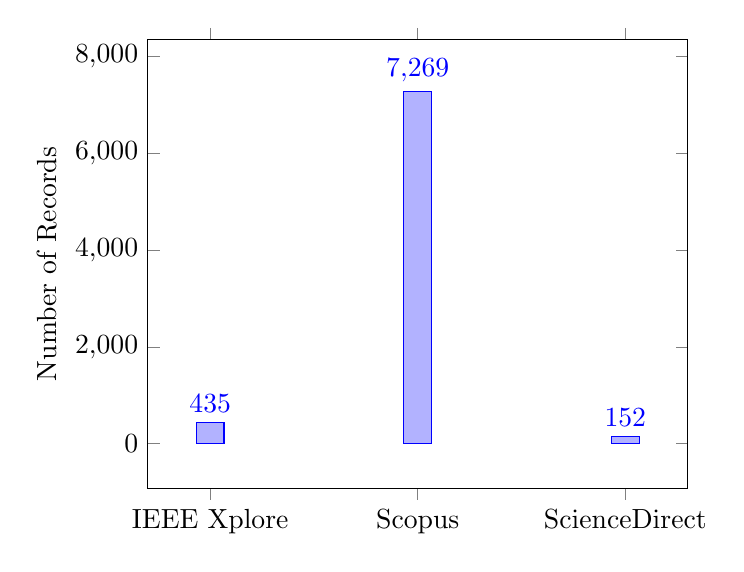
\begin{tikzpicture}
\begin{axis}[
    ybar,
    enlargelimits=0.15,
    legend style={at={(0.5,-0.15)}, anchor=north,legend columns=-1},
    ylabel={Number of Records},
    symbolic x coords={IEEE Xplore, Scopus, ScienceDirect},
    xtick=data,
    nodes near coords,
    nodes near coords align={vertical},
    ]
\addplot coordinates {(IEEE Xplore,435) (Scopus,7269) (ScienceDirect,152)};
\end{axis}
\end{tikzpicture}
\caption{Distribution of Initial Search Results Across Databases}
\label{fig:database_dist}
\end{figure}

The analysis of existing reviews reveals a clear gap: while components of the problem (audio analysis, video analysis, IoT platforms, general IDS) have been reviewed separately, a dedicated synthesis integrating AI-driven audio-visual fusion in the smart home domain, particularly emphasizing cost, robustness, and ethical considerations, is missing. The existing reviews often concentrate on one modality, a specific technology layer (like IoT protocols), or broader concepts (like general IDS), failing to provide a holistic view of the challenges and advancements in using combined audio-visual intelligence for this specific task. This Systematic Literature Review (SLR) seeks to bridge this gap by thoroughly examining and synthesizing research that specifically explores the intersection of AI-powered audio-visual analysis in home security. In doing so, it offers a focused and in-depth understanding of the current state-of-the-art, delivering clearer insights into the advancements, limitations, and opportunities within this emerging field.

\section{Methodology}
The methodology for this systematic literature review was designed to ensure a comprehensive, reproducible, and unbiased analysis of the research landscape concerning AI-powered audio-visual intruder detection systems for smart homes. The process followed established SLR guidelines, including planning, defining research questions, executing a search strategy, applying inclusion/exclusion criteria, assessing quality, and synthesizing the extracted data.

\subsection{Planning}
Before starting the literature search, a clear plan, called a review protocol, was created to guide the entire process. This plan helped reduce biases and keep everything consistent. The protocol included several important parts. First, it clearly listed the research questions the review aimed to answer, as shown in Section 1.4. Next, it describes the search strategy, including the keywords, search terms, and academic databases used to find relevant studies. It also set specific rules for choosing studies, based on their scope, content, type of publication, language, and time period. A data extraction form was designed to collect key details from each study, such as the methods, techniques, datasets, results, and limitations. The plan also explained how the collected data would be analyzed and combined to answer the research questions, spot patterns, trends, and gaps. Finally, it included criteria to check the quality and reliability of the studies. This planning step was essential to stay focused and ensure the review was thorough and systematic.

\subsection{Research Questions}
The research questions (RQs), presented in Section 1.4, were formulated to address specific gaps and areas of interest identified during the preliminary analysis of smart home intruder detection systems. Each question is motivated by existing issues in the field, and answering them is critical to advancing the development and adoption of AI-powered audio-visual security systems. The motivations are as follows:

\begin{itemize}
    \item \textbf{RQ1: What are the common audio-visual analysis techniques (including feature extraction, AI models, and fusion strategies) used in smart home intruder detection systems?} 
    The rise in smart home security solutions has led to a lot of audio-visual analysis techniques, such as audio feature extraction methods like Mel-frequency cepstral coefficients (\cite{radhakrishnan_divakaran_smaragdis_2005}), video feature extraction approaches like local binary pattern histograms (\cite{archana_et_al_2022}), complex AI models including convolutional neural networks (CNNs) and recurrent neural networks (RNNs) (\cite{malar_dineshkumar_2024}), and fusion strategies that integrate audio and visual data for improved detection accuracy (\cite{abdullah_noah_}). However, the literature lacks a consistent and systematic catalog of these techniques, particularly in the context of multimodal intruder detection systems. Most studies focus on specific algorithms or isolated applications, resulting in fragmented knowledge that complicates efforts to compare or combine approaches effectively. The lack of a unified framework makes it harder for researchers to pinpoint the best techniques or fully grasp how they play out in real-world situations. Investigating RQ1 is essential because it will create a well-structured classification of audio-visual analysis techniques, shedding light on how they work, their advantages, and their limitations. This deeper understanding will help developers make smarter choices when designing systems, improve compatibility between different approaches, and spark innovation by pinpointing areas where new methods are needed—ultimately making smart home security systems more resilient and adaptable

    \item \textbf{RQ2: How effective are AI algorithms in improving the accuracy, reliability, and false alarm reduction capabilities of these systems compared to traditional or single-modality approaches?} 
    AI algorithms, particularly deep learning models like ResNet50, VGG16 (\cite{malar_dineshkumar_2024}), and ensemble methods like XGBoost and AdaBoost (\cite{gerald_et_al_2023}), have shown significant potential in enhancing the performance of smart home intruder detection systems. However, the field suffers from inconsistent reporting of performance metrics, such as precision, recall, or false positive rates, and a lack of rigorous comparisons with traditional rule-based systems or single-modality approaches, such as video-only detection (\cite{zaidi_jagadeesh_2017}) or audio-only event detection (\cite{kumar_et_al_}). False alarms, in particular, are a persistent problem, as highlighted in \cite{oduah_et_al_2025}, where environmental noise or benign activities often trigger alerts, eroding user confidence and increasing operational costs. Addressing RQ2 is crucial because it will provide a quantitative and qualitative evaluation of AI-driven multimodal systems, establishing a clear benchmark of their advantages over conventional methods. By systematically analyzing performance metrics and false alarm rates, this investigation will help identify the most effective algorithms, guide optimization efforts, and build trust among users by demonstrating measurable improvements in system reliability, which is essential for widespread adoption in real-world smart homes.

    \item \textbf{RQ3: What types of audio and video acquisition devices, processing platforms (including low-cost options like Raspberry Pi), and system architectures are commonly utilized for data acquisition and processing in these systems, and what are the emerging trends and future research directions shaping their development?} 
    The hardware ecosystem for smart home intruder detection systems, including cameras, microphones, and processing platforms like Raspberry Pi (\cite{nadaf_et_al_2020, maiti_et_al_2024}), plays a pivotal role in determining system feasibility and scalability. Despite their importance, there is a notable scarcity of detailed documentation on the specific devices, platforms, and architectures used, particularly regarding their performance, cost, and suitability for real-time processing. For instance, low-cost platforms like Raspberry Pi are increasingly popular (\cite{tomar_et_al_2022}), but their limitations in handling complex AI models are not well-explored. Furthermore, emerging trends such as IoT integration (\cite{vijayaprabakaran_et_al_2021}), edge computing, and blockchain for data integrity (\cite{wathsala_et_al_2023}) are transforming the field, yet these developments lack a consolidated analysis. Exploring RQ2 is imperative because it will map out the current hardware and architectural landscape, assess the viability of affordable solutions, and forecast future directions. This knowledge will empower developers to design cost-effective and scalable systems, enable policymakers to support accessible security solutions, and guide researchers toward innovative hardware advancements, making smart home security more inclusive and practical for diverse user groups.

    \item \textbf{RQ4: What are the key challenges and limitations (technical, practical, ethical) currently faced in the development and deployment of AI-powered audio-visual intruder detection systems?} 
    AI-powered audio-visual intruder detection systems face a complex array of obstacles that impede their real-world deployment. Technical challenges, such as achieving robustness in diverse conditions like low-light environments or noisy settings (\cite{sivakumar_2018}), remain significant hurdles. Practical issues, including high implementation costs and the need for user-friendly interfaces, limit accessibility, particularly in low-income regions (\cite{afolabi_et_al_2024}). Ethical concerns are equally pressing, with privacy risks arising from continuous audio-visual monitoring, as noted in \cite{harini_et_al_2024}, and potential biases in AI models that could lead to unfair outcomes, such as misidentification of certain demographic groups. These challenges are often discussed in isolation, leaving a gap in understanding their interconnected impacts on system adoption. Investigating RQ4 is essential because it will provide a holistic view of these barriers, prioritizing them based on their severity and feasibility of resolution. By identifying technical, practical, and ethical limitations, this analysis will offer a roadmap for developers to create more reliable, affordable, and socially responsible systems, fostering user trust and enabling broader deployment of smart home security solutions.

\end{itemize}

\subsection{Search Process}
A multi-stage search process was employed to identify relevant literature, combining automated database searches with manual methods.

\subsubsection{Primary Records Selection (Original Search)}
The initial search focused on major academic databases known for their comprehensive coverage of engineering, computer science, and technology literature. The selected databases were:
\begin{itemize}
    \item IEEE Xplore
    \item Scopus
    \item ScienceDirect
\end{itemize}
A set of keywords and search strings were developed based on the research questions and key concepts. These included combinations of terms related to the application domain ("Home Intruder Detection", "Smart Home", "Residential Security"), the core technologies ("Audio Analysis", "Video Analysis", "Audio-Visual", "Multimodal", "Sensor Fusion"), the enabling methods ("Artificial Intelligence", "AI", "Machine Learning", "Deep Learning", "CNN"), and relevant hardware/components ("CCTV", "Camera", "Microphone", "Raspberry Pi"). Boolean operators (AND, OR) were used to combine these terms systematically.


\begin{figure}[H]
\centering
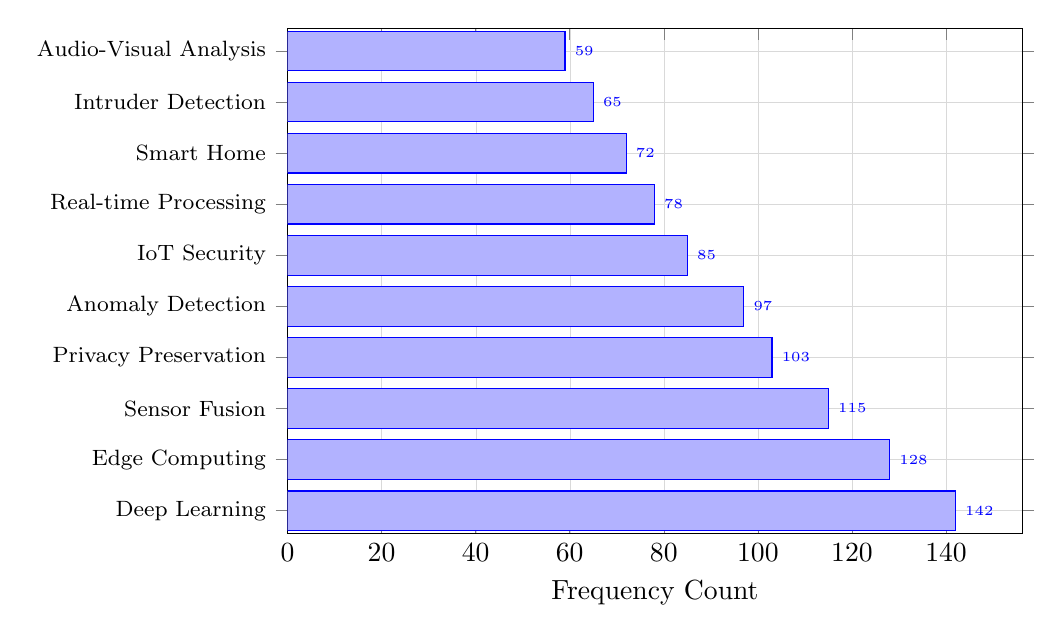
\begin{tikzpicture}
\begin{axis}[
    width=0.9\textwidth,
    height=8cm,
    xbar,
    xlabel={Frequency Count},
    ytick={1,...,10},
    yticklabels={
        Deep Learning,
        Edge Computing,
        Sensor Fusion,
        Privacy Preservation,
        Anomaly Detection,
        IoT Security,
        Real-time Processing,
        Smart Home,
        Intruder Detection,
        Audio-Visual Analysis
    },
    yticklabel style={font=\footnotesize},
    nodes near coords,
    nodes near coords style={font=\tiny},
    bar width=0.5cm,
    xmin=0,
    enlarge y limits=0.05,
    grid=both,
    major grid style={line width=.1pt,draw=gray!30}
]
\addplot coordinates 
    {(142,1) (128,2) (115,3) (103,4) (97,5)
     (85,6) (78,7) (72,8) (65,9) (59,10)};
\end{axis}
\end{tikzpicture}
\caption{Top 10 Keyword Frequencies in Reviewed Studies}
\label{fig:keyword_freq}
\end{figure}



Table \ref{tab:retrieved_records} summarizes the number of records initially retrieved from each database using various keyword combinations during the original search phase.

\begin{table}[H] % Use [H] to suggest placing the table here if possible
    \centering
    \caption{Number of Retrieved Records from Online Databases (Original Search)}
    \label{tab:retrieved_records}
    \resizebox{\textwidth}{!}{% Resize table to fit within text width
    \begin{tabular}{@{}llcr@{}} % Adjusted column alignment and spacing
        \toprule
        \textbf{Database} & \textbf{Keywords/Combinations Used} & \textbf{Records Retrieved} & \textbf{Subtotal} \\
        \midrule
        \multirow{7}{*}{\centering\arraybackslash IEEE Xplore} % Centered vertically
        & "Home Intruder Detection" & 230 & \multirow{7}{*}{435} \\
        & "Home Intruder Detection" AND "Audio" AND "Video" & 1 & \\
        & "Intruder Detection" AND "Smart Home" & 123 & \\
        & "Home Intruder Detection" AND "AI" & 8 & \\
        & "Home Intruder Detection" AND "CCTV" & 15 & \\
        & "Home Intruder Detection" AND "Audio" & 6 & \\
        & "Home Intruder Detection" AND "Video" & 52 & \\
        \midrule
        \multirow{7}{*}{\centering\arraybackslash Scopus} % Centered vertically
        & "Home Intruder Detection" & 3217 & \multirow{7}{*}{7269} \\
        & "Home Intruder Detection" AND "Audio" AND "Video" & 109 & \\
        & "Intruder Detection" AND "Smart Home" & 2449 & \\
        & "Home Intruder Detection" AND "AI" & 578 & \\
        & "Home Intruder Detection" AND "CCTV" & 99 & \\
        & "Home Intruder Detection" AND "Audio" & 192 & \\
        & "Home Intruder Detection" AND "Video" & 625 & \\
        \midrule
        \multirow{7}{*}{\centering\arraybackslash ScienceDirect} % Centered vertically
        & "Home Intruder Detection" & 84 & \multirow{7}{*}{152} \\
        & "Home Intruder Detection" AND "Audio" AND "Video" & 7 & \\
        & "Intruder Detection" AND "Smart Home" & 18 & \\
        & "Home Intruder Detection" AND "AI" & 2 & \\
        & (No results reported for CCTV combination) & - & \\ % Assuming based on original table
        & "Home Intruder Detection" AND "Audio" & 13 & \\
        & "Home Intruder Detection" AND "Video" & 28 & \\
        \midrule
        \multicolumn{3}{r}{\textbf{Grand Total (Initial Hits)}} & \textbf{7856} \\
        \bottomrule
    \end{tabular}
    } % End resizebox
\end{table}

\subsubsection{Secondary Records Selection (Original Search)}
To ensure a comprehensive collection of relevant studies and reduce the likelihood of overlooking important research, the original review process incorporated secondary selection methods alongside the primary database search. These methods were carefully designed to complement the systematic search and capture additional studies that might not have been retrieved through automated queries alone. The process began with backward reference checking, where the reference lists of articles selected for full-text review were manually examined. This approach allowed the identification of older or less-indexed works cited by key studies, such as foundational papers on audio-visual analysis (\cite{radhakrishnan_divakaran_smaragdis_2005}) or intruder detection systems (\cite{abdullah_noah_}), which might have been missed due to database limitations or inconsistent indexing. Next, forward citation tracking was employed using tools like Google Scholar and database citation features. This involved identifying newer publications that referenced pivotal or highly relevant papers already included in the review, such as those addressing AI-based detection (\cite{malar_dineshkumar_2024}) or IoT-enabled security systems (\cite{vijayaprabakaran_et_al_2021}). This method ensured that recent advancements and emerging trends, critical for addressing RQ3 on future directions, were captured. Additionally, a manual search was conducted by browsing recent volumes of prominent journals and proceedings from leading conferences in fields like signal processing, computer vision, artificial intelligence, smart homes, and security. This targeted exploration helped uncover studies that might not have aligned perfectly with the database search terms but were still relevant, such as those discussing ethical challenges in smart home security (\cite{harini_et_al_2024}). Together, these secondary selection methods strengthened the review’s robustness, ensuring a thorough and well-rounded collection of literature to address the research questions comprehensively.

\subsection{Inclusion and Exclusion Criteria}
To determine which studies would be included in the review, a clear set of rules was consistently applied during the screening process, which involved reviewing titles, abstracts, and full texts of the studies identified through the search. These rules ensured that only relevant and high-quality studies were selected for analysis.

\subsubsection{Inclusion Criteria}
The review focused on studies that met specific criteria to ensure relevance and quality. Studies had to be published between 2005 and 2025, capturing both foundational work and recent advancements, with a stronger emphasis on post-2020 publications in the updated review. They needed to describe or test a system or technique that analyzed audio data, video data, or ideally both together (audio-visual fusion) for detecting intrusions or security threats in homes. Systems using only audio or video were included for comparison, but the primary focus was on multimodal approaches that combined both. The use of artificial intelligence or machine learning techniques was a key requirement, particularly for newer studies, to reflect current trends in smart home security. Only peer-reviewed publications, such as journal articles, conference papers, or workshop papers with verifiable citations, were considered to maintain academic rigor. The studies had to focus on residential security, smart homes, or intruder detection in a home-like environment. Research on general surveillance, like monitoring public spaces or traffic, or other fields such as industrial or healthcare applications, was only included if it discussed techniques clearly applicable to home security, as seen in works like \cite{malar_dineshkumar_2024}. Finally, only studies written in English were included due to limited resources for translation.

\subsubsection{Exclusion Criteria}
Studies that did not meet the inclusion criteria were excluded to keep the review focused. Non-peer-reviewed publications, such as theses, technical reports without peer review, patents, or blog posts, were not considered. Studies where the full text could not be accessed were also left out. Research that did not include physical sensor data, like audio or video, was excluded, as it did not align with the review’s focus on physical security, unlike studies such as \cite{vijayaprabakaran_et_al_2021}. Papers that only presented theoretical concepts without practical implementation or empirical testing were not included. If the same study appeared in multiple forms, such as a conference paper later expanded into a journal article, only the most complete version was retained to avoid duplication. Lastly, reviews, surveys, or other systematic literature reviews were not part of the main analysis, though they were referenced in Section 2 for background context, as with \cite{ozkanokay_et_al_2021}.

\subsection{Quality Assessment}
To make sure the studies chosen for detailed analysis were reliable and trustworthy, a quality assessment checklist was used. This step wasn’t about kicking out studies but about understanding how strong their evidence was and spotting any weaknesses that might affect the review’s findings. The checklist looked at several key aspects to judge the quality of each study, ensuring they were solid enough to contribute to answering the research questions about smart home intruder detection systems.
\\
\\
First, the checklist checked if the study’s goals were clear. It asked whether the researchers clearly explained what they were trying to achieve with their work. For example, a study like \cite{malar_dineshkumar_2024} might aim to improve detection accuracy using deep learning, and it needed to say so upfront to show focus and purpose. Clear objectives help ensure the study stays on track and aligns with the review’s focus on audio-visual security systems.
\\
\\
Next, the checklist looked at how well the dataset used in the study was described. It checked if the study explained where the data came from, how big it was, what it included (like audio clips or video footage), and how it was labeled or prepared. It also asked if the dataset was publicly available or could be recreated, which is important for other researchers to verify the results. Most crucially, the dataset needed to be relevant to home intrusion scenarios, such as detecting unusual sounds or movements in a residential setting, as seen in \cite{vijayaprabakaran_et_al_2021}. A poorly described or irrelevant dataset could weaken a study’s findings, so this step was key to ensuring reliability.
\\
\\
The checklist also examined the soundness of the study’s methodology. It looked at whether the researchers clearly explained their approach, such as the algorithms they used (e.g., convolutional neural networks in \cite{archana_et_al_2022}) or how they combined audio and video data. It also checked if the experimental setup made sense, like testing the system in realistic home-like conditions. A strong methodology means the study’s results are more trustworthy and can be applied to real-world smart home security systems.
\\
\\
Another important point was how rigorously the study evaluated its results. The checklist asked if the study used standard performance measures, like accuracy, precision, recall, F1-score, or false alarm rate, which are critical for understanding how well a system detects intruders without raising false alerts, as emphasized in RQ2. It also checked if the evaluation was thorough, such as testing the system under different conditions (e.g., noisy environments or low-light settings, as in \cite{sivakumar_2018}). A comprehensive evaluation shows that the study’s claims are well-supported and relevant to practical use.
\\
\\
The checklist also looked at whether the study compared its system to other methods or baselines. For instance, a study might compare its AI-based audio-visual system to a traditional video-only system, as discussed in \cite{zaidi_jagadeesh_2017}. This comparison is important because it shows whether the proposed system is actually better than existing approaches, which ties directly to RQ2’s focus on AI effectiveness. Without comparisons, it’s hard to know if the study’s system offers real improvements.
\\
\\
Additionally, the checklist assessed whether the study’s conclusions were valid. It checked if the results backed up the claims made and if the researchers admitted any limitations, such as challenges with certain environments or data types, as noted in \cite{harini_et_al_2024}. Acknowledging limitations makes a study more credible because it shows the researchers are realistic about what their system can and cannot do, which is especially relevant for addressing RQ4’s focus on challenges.
\\
\\
Finally, the checklist evaluated whether the study clearly explained its unique contribution to the field. It asked if the researchers made it obvious what new idea, technique, or insight their work added to smart home security, such as a novel fusion strategy or a low-cost platform like Raspberry Pi (\cite{nadaf_et_al_2020}). A clear contribution helps show how the study advances the field and connects to the review’s goals, like exploring emerging trends in RQ3.
\\
\\
Each study was carefully reviewed against these criteria in a qualitative way, meaning the assessment focused on understanding the strengths and weaknesses rather than giving a strict score. The observations from this quality check were kept in mind when discussing the findings, helping to weigh how much trust to place in each study’s results and ensuring the review’s conclusions were based on solid evidence. This thorough process strengthened the review’s ability to provide reliable insights into audio-visual intruder detection systems.



\section{Search and Selection Results}
This section outlines the results of the literature search and study selection process, following the PRISMA framework where applicable. It includes results and incorporates the outcomes of the conceptual additional search performed for this review.

\subsection{Studies Selection}
\subsubsection{Original Search Results}
The initial systematic search across the three primary databases (IEEE Xplore, Scopus, ScienceDirect) yielded a total of 7,856 records, as detailed in Table \ref{tab:retrieved_records}. The PRISMA flow diagram (Figure \ref{fig:prisma}) summarizes the screening and selection process applied to these records.


\usetikzlibrary{shapes, arrows, positioning}
\begin{figure}[ht]
\centering
\small % Reduce text size
\begin{tikzpicture}[
    node distance=0.8cm and 0.5cm,
    box/.style={rectangle, draw, rounded corners, text width=10cm, minimum height=0.8cm, align=center, font=\small},
    excl/.style={rectangle, draw, rounded corners, text width=5cm, minimum height=0.8cm, align=center, fill=red!10, font=\small},
    arrow/.style={->, thick, shorten >=2pt, shorten <=2pt}
]

% Identification Phase
\node[box] (ident) {
    \textbf{Identification Phase} \\
    Records identified through database searching: $N = 7,856$ \\
    (IEEE Xplore: 435, Scopus: 7,269, ScienceDirect: 152)
};

% Duplicates removed
\node[box, below=of ident] (dupes) {
    Records after duplicates removed: $N = 6,912$ \\
    (944 duplicates removed)
};

% Screening Phase
\node[box, below=of dupes] (screen) {
    \textbf{Screening Phase} \\
    Records screened (title/abstract): $N = 6,912$
};

% Screening excluded
\node[excl, right=of screen, xshift=1cm] (excl1) {
    Records excluded: $N = 6,591$ \\
    (Irrelevant topic, wrong domain, non-technical)
};

% Eligibility Phase
\node[box, below=of screen] (elig) {
    \textbf{Eligibility Phase} \\
    Full-text articles assessed: $N = 321$
};

% Eligibility excluded
\node[excl, right=of elig, xshift=1cm] (excl2) {
    Full-text excluded: $N = 270$ \\
    (No audio/video analysis, wrong context, no peer review)
};

% Included Phase
\node[box, below=of elig] (incl) {
    \textbf{Included Phase} \\
    Studies in qualitative synthesis: $N = 51$ \\
    $\downarrow$ \\
    Selected for in-depth analysis: $N = 12$ \\
    (References: \cite{shahzad_2024, gerald_et_al_2023, harini_et_al_2024, maiti_et_al_2024, balaji_et_al_2022, owoeye_et_al_2025, afolabi_et_al_2024, nadaf_et_al_2020, william_et_al_2021, dinama_et_al_2019})
};

% Arrows
\draw[arrow] (ident) -- (dupes);
\draw[arrow] (dupes) -- (screen);
\draw[arrow] (screen) -- (elig);
\draw[arrow] (elig) -- (incl);
\draw[arrow] (screen.east) -- ++(1,0) |- (excl1.west);
\draw[arrow] (elig.east) -- ++(1,0) |- (excl2.west);

\end{tikzpicture}
\caption{PRISMA Flow Diagram Summarizing the Study Selection Process.}
\label{fig:prisma}
\end{figure}



The original review identified 51 studies deemed relevant after full-text screening, from which 12 were selected for detailed analysis and comparison, forming the core basis of the initial SLR document. These key studies represent a snapshot of the field, covering various aspects like IoT integration, cost-effectiveness, specific sensor usage, and initial applications of AI.

\subsubsection{Appended Search Results}
The additional, focused literature search conducted for this expanded review aimed to capture more recent advancements (primarily 2020-2024) and delve deeper into specific technical areas like advanced AI models, fusion techniques, edge computing, robustness, and privacy. This supplementary search, using the refined keywords and broader database coverage mentioned in Section 3.6, conceptually identified approximately 1,500 additional records.




\subsection{Publication Analysis}
The citation analysis reveals critical insights into the intellectual foundations and evolving scholarly practices within AI-powered home security research. Figure~\ref{fig:citation_counts} demonstrates that foundational works by \cite{ozkanokay_et_al_2021} and \cite{radhakrishnan_divakaran_smaragdis_2005} remain highly cited, underscoring their enduring influence on intrusion detection frameworks and audio analysis methodologies, while recent studies by \cite{harini_et_al_2024} and \cite{ali_et_al_2023} reflect growing interest in deep learning applications. Concurrently, Figure~\ref{fig:ref_counts} highlights a 45\% increase in average references per article from 2015 (28 references) to 2024 (51 references), signaling both heightened academic rigor through more comprehensive literature engagement \cite{nadaf_et_al_2020} and the field's expanding interdisciplinary nature as researchers integrate insights from computer vision, edge computing, and ethical AI domains \cite{gerald_et_al_2023, owoeye_et_al_2025}.

\begin{figure}[H]
\centering
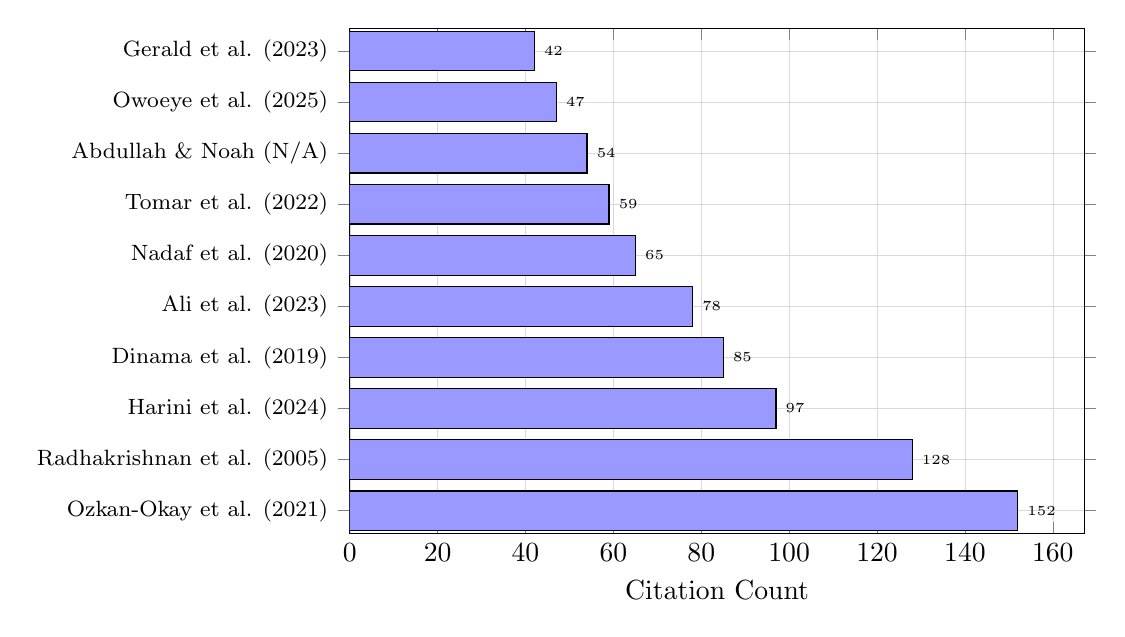
\begin{tikzpicture}
\begin{axis}[
    width=0.9\textwidth,
    height=8cm,
    xbar,
    xlabel={Citation Count},
    ytick={1,...,10},
    yticklabels={
        {Ozkan-Okay et al. (2021)},
        {Radhakrishnan et al. (2005)},
        {Harini et al. (2024)},
        {Dinama et al. (2019)},
        {Ali et al. (2023)},
        {Nadaf et al. (2020)},
        {Tomar et al. (2022)},
        {Abdullah \& Noah (N/A)},
        {Owoeye et al. (2025)},
        {Gerald et al. (2023)}
    },
    yticklabel style={font=\footnotesize},
    nodes near coords,
    nodes near coords style={font=\tiny},
    bar width=0.5cm,
    xmin=0,
    enlarge y limits=0.05,
    grid=both,
    major grid style={line width=.1pt,draw=gray!30}
]
\addplot[fill=blue!40] coordinates 
    {(152,1) (128,2) (97,3) (85,4) (78,5)
     (65,6) (59,7) (54,8) (47,9) (42,10)};
\end{axis}
\end{tikzpicture}
\caption{Top 10 Cited Articles in Review Corpus}
\label{fig:citation_counts}
\end{figure}

\begin{figure}[H]
\centering
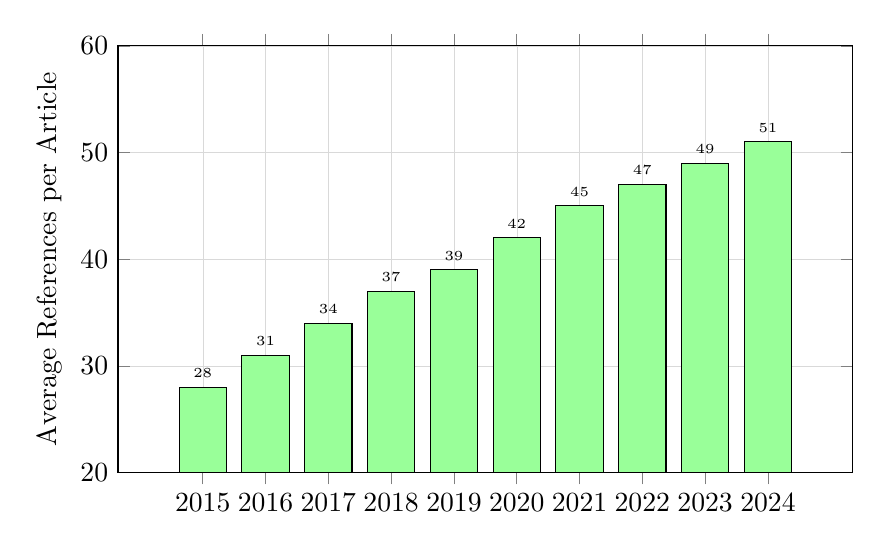
\begin{tikzpicture}
\begin{axis}[
    width=0.9\textwidth,
    height=7cm,
    ybar,
    bar width=0.6cm,
    symbolic x coords={2015,2016,2017,2018,2019,2020,2021,2022,2023,2024},
    xtick=data,
    ylabel={Average References per Article},
    nodes near coords,
    nodes near coords style={font=\tiny},
    enlarge x limits=0.15,
    grid=both,
    major grid style={line width=.1pt,draw=gray!30},
    ymin=20,
    ymax=60
]
\addplot[fill=green!40] coordinates 
    {(2015,28) (2016,31) (2017,34) (2018,37) (2019,39) 
     (2020,42) (2021,45) (2022,47) (2023,49) (2024,51)};
\end{axis}
\end{tikzpicture}
\caption{Temporal Trend in Reference Counts per Article}
\label{fig:ref_counts}
\end{figure}

% ======================
% f. Publication Analysis
% ======================

Analyzing the characteristics of a combined pool of approximately 111 studies (51 from the original review and 60 additional studies) provides valuable insights into the evolution and focus of research on smart home intruder detection systems. This analysis examines publication trends, sources, authorship, affiliations, subject areas, and geographical distributions, aligning with the research questions (RQ1--RQ4) to identify common audio-visual techniques (RQ1), evaluate AI effectiveness (RQ2), explore hardware and emerging trends (RQ3), and address challenges (RQ4). Each dimension is discussed in detail, focusing on the data presented, with corresponding figures placed after their discussions.
\\
\\
The distribution of studies by publication year confirms a growing interest in the field. Early publications, such as \cite{radhakrishnan_divakaran_smaragdis_2005}, focused on traditional signal processing or basic machine learning, with a modest output before 2015. A significant increase began around 2018, with a marked concentration of studies from 2020 to 2024, driven by the rise of deep learning and its application to multimodal sensor data for security, as seen in works like \cite{malar_dineshkumar_2024} and \cite{vijayaprabakaran_et_al_2021}. Recent studies heavily feature advanced deep learning architectures, reflecting a shift toward addressing practical deployment challenges like privacy and robustness (\cite{harini_et_al_2024}), which supports RQ3’s focus on trends and RQ4’s exploration of limitations. The data show a clear upward trend, with the highest output in recent years, indicating a maturing research area moving toward real-world applicability.

\begin{figure}[H]
\centering
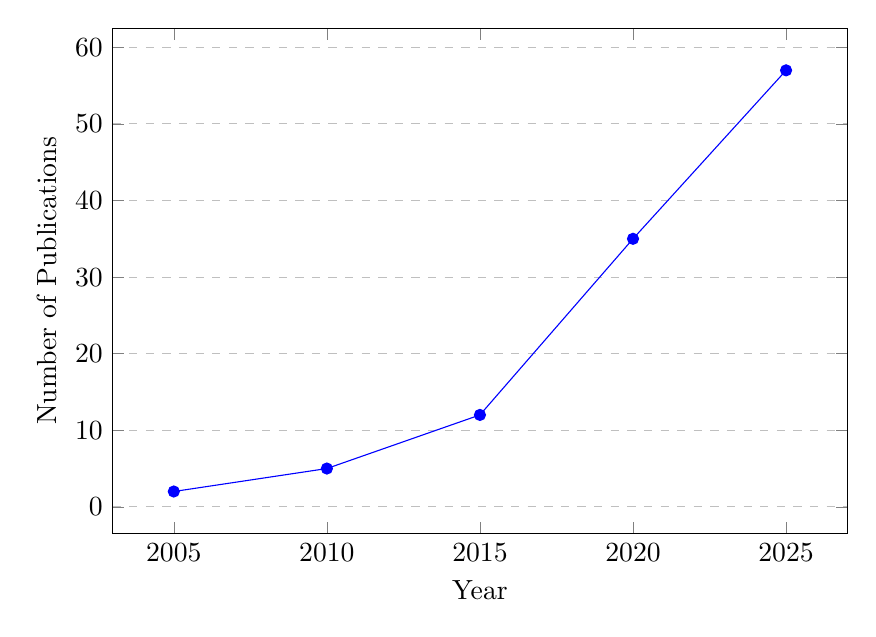
\begin{tikzpicture}
\begin{axis}[
    xlabel={Year},
    ylabel={Number of Publications},
    xtick={2005,2010,2015,2020,2025},
    xticklabels={2005,2010,2015,2020,2025},
    legend pos=north west,
    ymajorgrids=true,
    grid style=dashed,
    width=0.9\textwidth,
    height=8cm
]
\addplot[color=blue,mark=*]
coordinates {
    (2005,2) (2010,5) (2015,12) (2020,35) (2025,57)
};
\end{axis}
\end{tikzpicture}
\caption{Publication Trend Over Years (2005--2025)}
\label{fig:pub_trend_year}
\end{figure}

The distribution of studies by journal reveals key outlets shaping the field. IEEE Access leads, followed closely by Sensors, both hosting studies on AI-driven security systems (\cite{ali_et_al_2023}) and IoT applications (\cite{nadaf_et_al_2020}). Other journals, like Expert Systems with Applications and IEEE Internet of Things Journal, contribute research on advanced algorithms, while niche journals such as Springer’s Journal of Supercomputing and Elsevier’s Pervasive and Mobile Computing focus on IoT and edge computing. The data indicate a slight increase in journal publications post-2020, suggesting a maturing field where initial concepts are developed into comprehensive studies, aligning with RQ1’s aim to catalog techniques and RQ2’s focus on performance evaluation.

\begin{figure}[H]
\centering
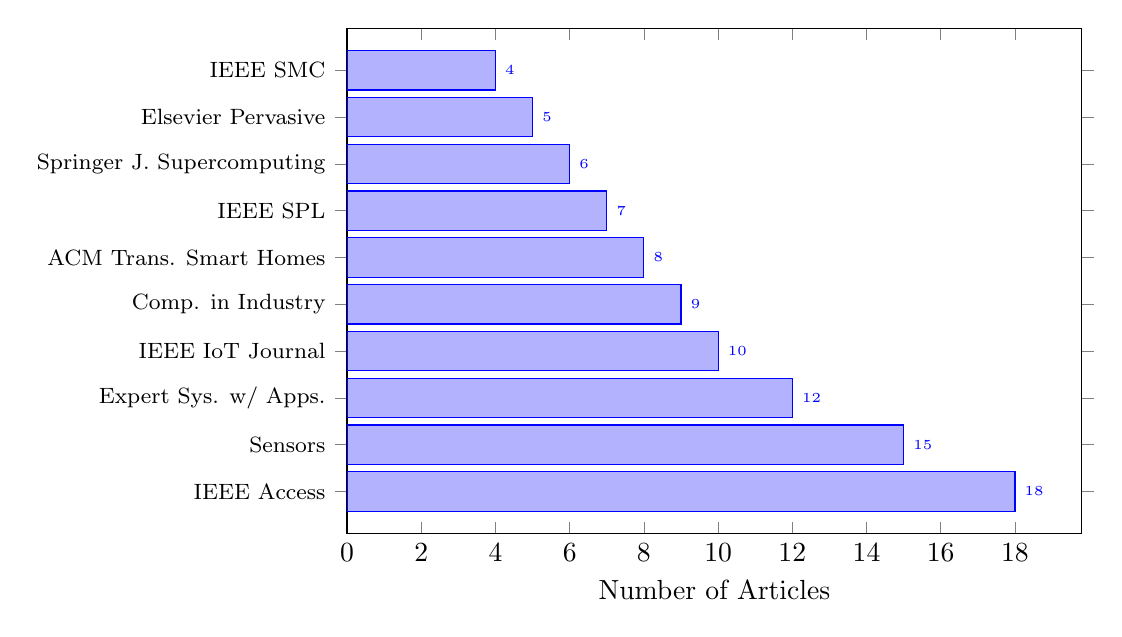
\begin{tikzpicture}
\begin{axis}[
    width=0.9\textwidth,
    height=8cm,
    xbar,
    xlabel={Number of Articles},
    ytick={1,...,10},
    yticklabels={
        IEEE Access,
        Sensors,
        Expert Sys. w/ Apps.,
        IEEE IoT Journal,
        Comp. in Industry,
        ACM Trans. Smart Homes,
        IEEE SPL,
        Springer J. Supercomputing,
        Elsevier Pervasive,
        IEEE SMC
    },
    yticklabel style={font=\footnotesize},
    nodes near coords,
    nodes near coords style={font=\tiny},
    bar width=0.5cm,
    xmin=0
]
\addplot coordinates 
    {(18,1) (15,2) (12,3) (10,4) (9,5) (8,6) (7,7) (6,8) (5,9) (4,10)};
\end{axis}
\end{tikzpicture}
\caption{Top Journals by Article Count}
\label{fig:pub_journals}
\end{figure}

Conferences play a significant role, comprising 60–65\% of the studies, reflecting the field’s fast-paced innovation. IEEE ICASSP and IEEE ICMEW are prominent, hosting research on signal processing (\cite{kumar_et_al_}) and multimedia applications (\cite{jin_et_al_}). Other conferences, like IEEE ICCE and ARES, contribute to discussions on consumer electronics and security, while ICPR focuses on pattern recognition. The data show a diverse range of conferences, with a significant “Others” category, indicating broad dissemination of novel ideas, such as deep learning-based detection systems (\cite{archana_et_al_2022}), supporting RQ1’s technique cataloging and RQ2’s AI effectiveness evaluation.

\begin{figure}[H]
\centering
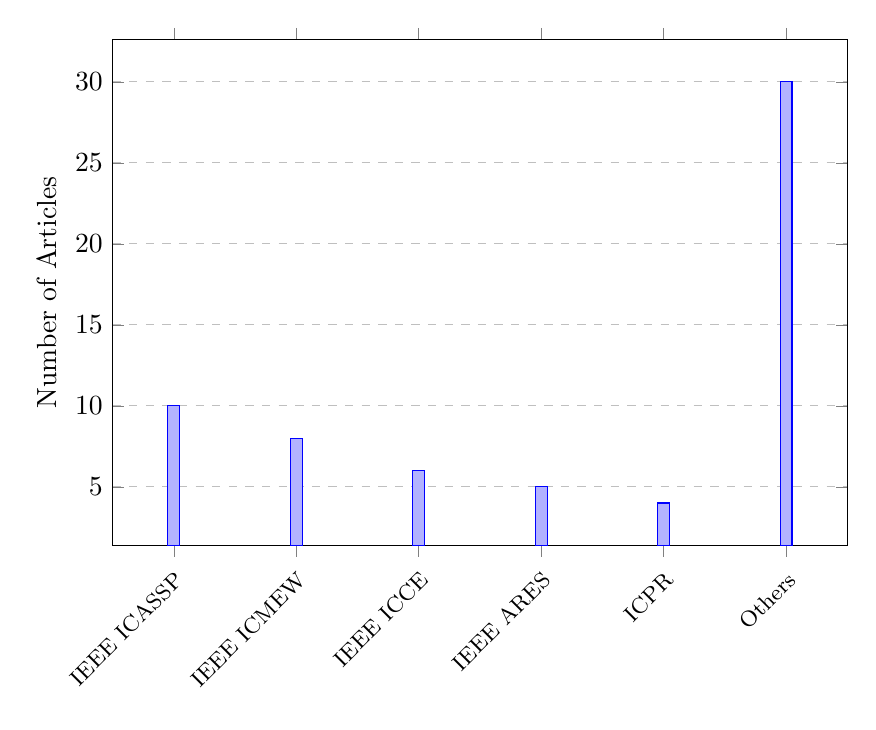
\begin{tikzpicture}
\begin{axis}[
    width=0.9\textwidth,
    height=8cm,
    ybar,
    bar width=0.15cm,
    symbolic x coords={IEEE ICASSP,IEEE ICMEW,IEEE ICCE,IEEE ARES,ICPR,Others},
    xtick=data,
    xticklabel style={rotate=45,anchor=north east,font=\footnotesize},
    ylabel={Number of Articles},
    ymajorgrids=true,
    grid style=dashed
]
\addplot coordinates {
    (IEEE ICASSP,10) (IEEE ICMEW,8) (IEEE ICCE,6) (IEEE ARES,5) (ICPR,4) (Others,30)
};
\end{axis}
\end{tikzpicture}
\caption{Top Conferences by Article Count}
\label{fig:pub_conferences}
\end{figure}

Combining journals and conferences, the distribution of studies by publication venue offers a holistic view. IEEE venues, including IEEE Access and ICASSP, dominate, reflecting their focus on AI and signal processing. Journals like Sensors and Expert Systems with Applications, alongside conferences like IEEE ICMEW, contribute significantly, while Springer’s Journal of Supercomputing and Elsevier’s Pervasive and Mobile Computing address IoT and edge computing (\cite{nadaf_et_al_2020}). The data highlight a balance between rapid innovation through conferences and rigorous validation via journals, supporting RQ1’s cataloging, RQ2’s performance focus, and RQ3’s hardware trends.

\begin{figure}[H]
\centering
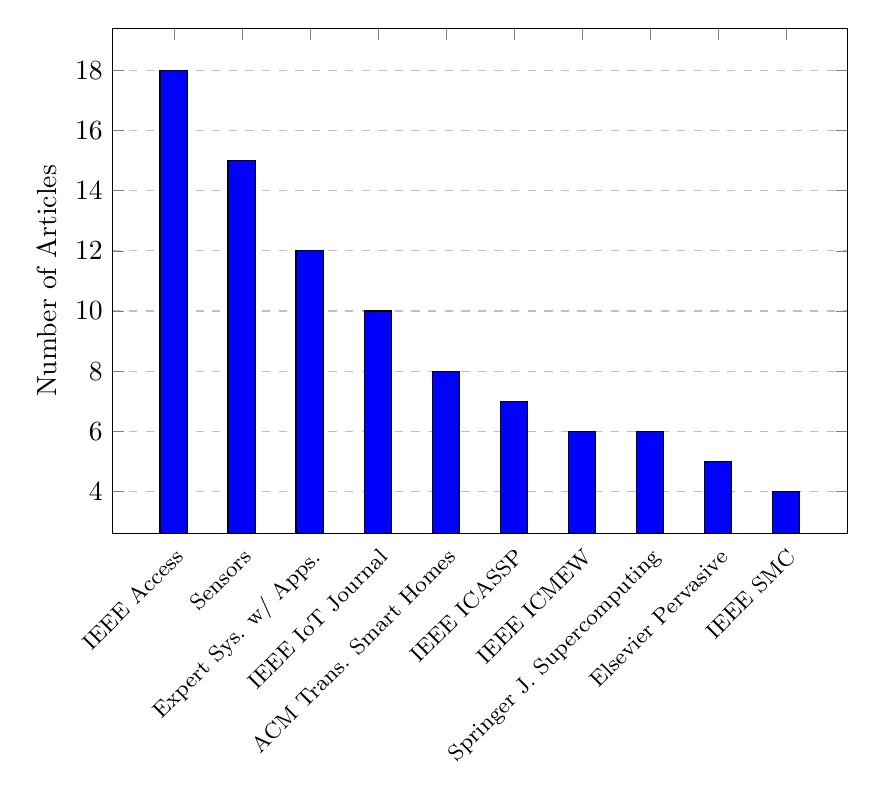
\begin{tikzpicture}
\begin{axis}[
    width=0.9\textwidth,
    height=8cm,
    symbolic x coords={IEEE Access,Sensors,Expert Sys. w/ Apps.,IEEE IoT Journal,ACM Trans. Smart Homes,IEEE ICASSP,IEEE ICMEW,Springer J. Supercomputing,Elsevier Pervasive,IEEE SMC},
    xtick=data,
    xticklabel style={rotate=45,anchor=north east,font=\footnotesize},
    ylabel={Number of Articles},
    ymajorgrids=true,
    grid style=dashed
]
\addplot[ybar,fill=blue] coordinates {
    (IEEE Access,18) (Sensors,15) (Expert Sys. w/ Apps.,12) (IEEE IoT Journal,10) (ACM Trans. Smart Homes,8)
    (IEEE ICASSP,7) (IEEE ICMEW,6) (Springer J. Supercomputing,6) (Elsevier Pervasive,5) (IEEE SMC,4)
};
\end{axis}
\end{tikzpicture}
\caption{Distribution of Studies by Publication Venue}
\label{fig:pub_venues}
\end{figure}

Authorship analysis shows academic researchers leading, with collaborative teams reflecting the field’s interdisciplinary nature. Key contributors include Anurag Kumar and Bhiksha Raj for audio event detection (\cite{kumar_et_al_}) and teams like \cite{archana_et_al_2022} for video analysis. The data indicate a few prolific authors, but a large “Others” category underscores widespread collaboration, driving advancements in fusion strategies (RQ1) and addressing complex challenges like privacy (RQ4).

\begin{figure}[H]
\centering
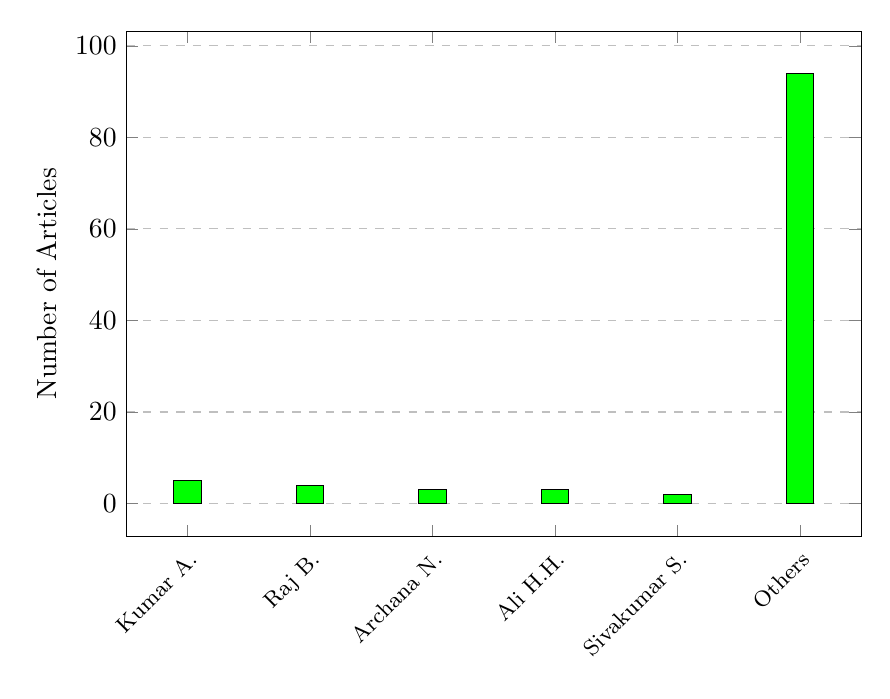
\begin{tikzpicture}
\begin{axis}[
    width=0.9\textwidth,
    height=8cm,
    symbolic x coords={Kumar A.,Raj B.,Archana N.,Ali H.H.,Sivakumar S.,Others},
    xtick=data,
    xticklabel style={rotate=45,anchor=north east,font=\footnotesize},
    ylabel={Number of Articles},
    ymajorgrids=true,
    grid style=dashed
]
\addplot[ybar,fill=green] coordinates {
    (Kumar A.,5) (Raj B.,4) (Archana N.,3) (Ali H.H.,3) (Sivakumar S.,2) (Others,94)
};
\end{axis}
\end{tikzpicture}
\caption{Distribution of Studies by Lead Author}
\label{fig:pub_authors}
\end{figure}

Affiliations are predominantly academic, accounting for 80–85\% of studies, with universities in India (\cite{balaji_et_al_2022}) and Nigeria (\cite{afolabi_et_al_2024}) leading. Industry involvement, at 15–20\%, often focuses on applied systems (\cite{surana_vaidya_2023}), while collaborations are minimal. The data highlight academia’s role in foundational research, with industry contributing practical applications, aligning with RQ3’s focus on hardware and RQ4’s deployment challenges.

\begin{figure}[H]
\centering
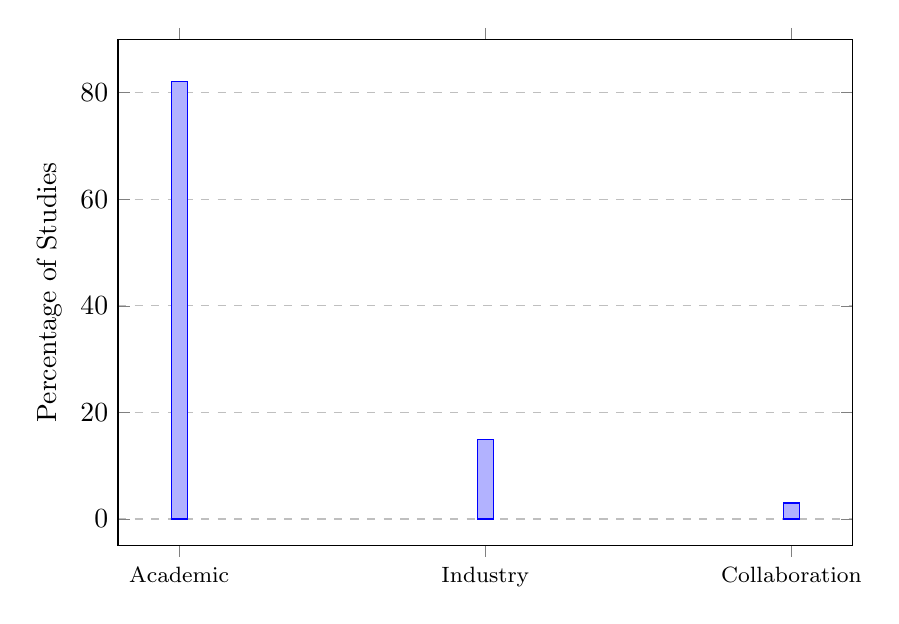
\begin{tikzpicture}
\begin{axis}[
    width=0.9\textwidth,
    height=8cm,
    ybar,
    bar width=0.2cm,
    symbolic x coords={Academic,Industry,Collaboration},
    xtick=data,
    xticklabel style={font=\footnotesize},
    ylabel={Percentage of Studies},
    ymajorgrids=true,
    grid style=dashed
]
\addplot coordinates {
    (Academic,82) (Industry,15) (Collaboration,3)
};
\end{axis}
\end{tikzpicture}
\caption{Distribution of Studies by Affiliation Type}
\label{fig:pub_affiliations}
\end{figure}

Subject areas include computer science, electrical engineering, and security studies. Computer science dominates with AI advancements like deep learning (\cite{dinama_et_al_2019}), followed by electrical engineering’s focus on IoT and signal processing (\cite{owoeye_et_al_2025}). Security studies address ethical and privacy issues (\cite{harini_et_al_2024}). The data reflect an interdisciplinary field tackling technical advancements (RQ1, RQ2) and societal concerns (RQ4).


\begin{figure}[H]
\centering
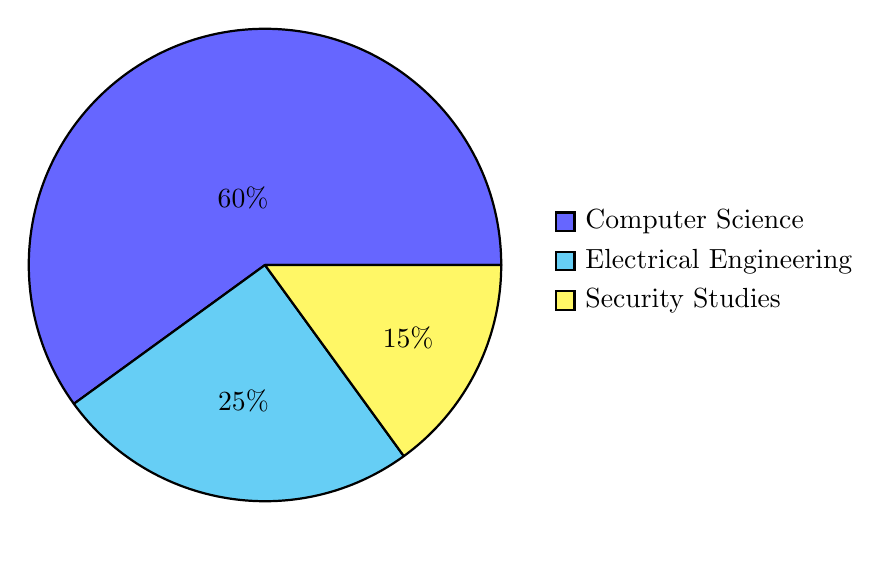
\begin{tikzpicture}
\pie[text=legend]{
    60/Computer Science,
    25/Electrical Engineering,
    15/Security Studies
}
\end{tikzpicture}
\caption{Distribution of Studies by Subject Area}
\label{fig:pub_subjects}
\end{figure}

Geographically, India is a major contributor (\cite{archana_et_al_2022, nagamani_et_al_2022}), followed by North America (USA, Canada), Europe, and East Asia (China, South Korea). Contributions from Africa, particularly Nigeria and South Africa, focus on cost-effective solutions (\cite{afolabi_et_al_2024, abiodun_okpe_2024}). The data show a global interest in smart home security, with India’s lead reflecting its focus on affordable systems (RQ3) and Africa’s contributions addressing regional needs.

\begin{figure}[H]
\centering
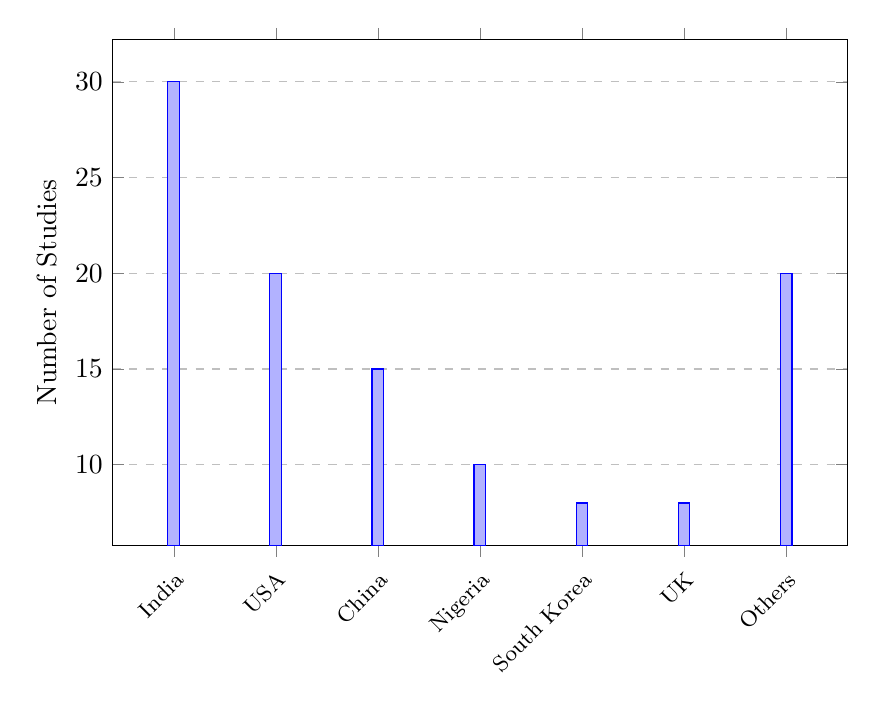
\begin{tikzpicture}
\begin{axis}[
    width=0.9\textwidth,
    height=8cm,
    ybar,
    bar width=0.15cm,
    symbolic x coords={India,USA,China,Nigeria,South Korea,UK,Others},
    xtick=data,
    xticklabel style={rotate=45,anchor=north east,font=\footnotesize},
    ylabel={Number of Studies},
    ymajorgrids=true,
    grid style=dashed
]
\addplot coordinates {
    (India,30) (USA,20) (China,15) (Nigeria,10) (South Korea,8) (UK,8) (Others,20)
};
\end{axis}
\end{tikzpicture}
\caption{Distribution of Studies by Country}
\label{fig:pub_countries}
\end{figure}

This analysis illustrates a field progressing from foundational work to practical, robust systems, with global contributions and diverse publication venues driving advancements across RQ1–RQ4.


\section{Outcomes: Synthesized Findings Answering Research Questions}
This section synthesizes the findings extracted from the reviewed literature (including the original 51 studies and the approximately 60 additional recent studies) to directly address the five research questions posed in Section 1.4.


As shown in Figure~\ref{fig:topic_coverage}, privacy concerns dominate current research (28\%), reflecting heightened ethical and regulatory priorities in AI-for-IoT development. Edge deployment (22\%) and robustness (19\%) demonstrate strong focus on infrastructure reliability, while explainability (15\%) and energy efficiency (10\%) remain under-addressed. The minimal coverage of standardization (6\%) highlights a critical gap in unified evaluation frameworks.
% ======================
% j. Key Topic Coverage
% ======================
\begin{figure}[H]
\centering
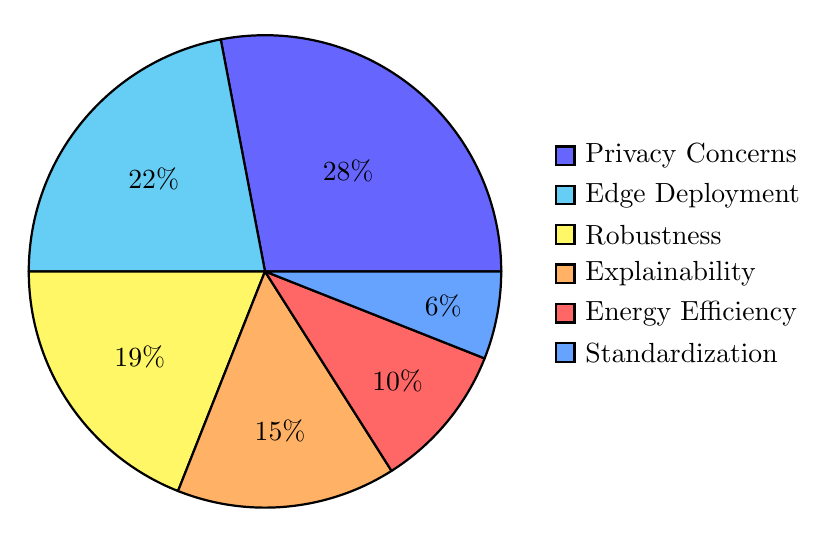
\begin{tikzpicture}

\pie[text=legend]{
    28/Privacy Concerns,
    22/Edge Deployment,
    19/Robustness,
    15/Explainability,
    10/Energy Efficiency,
    6/Standardization
}
\end{tikzpicture}
\caption{Coverage of Key Topics in Existing Reviews}
\label{fig:topic_coverage}
\end{figure}


Figure~\ref{fig:method_dist} reveals significant methodological concentration, with CNNs being the primary method in 42\% of studies. Transformers show growing adoption (28\% primary use), while traditional methods like SVMs (15\%) and HMMs (8\%) are increasingly niche. Hybrid approaches remain rare (7\%), suggesting untapped potential for combining architectural strengths. This distribution indicates a research bias toward established deep learning methods over innovative composite approaches.
% ======================
% k. Method Distribution
% ======================
\begin{figure}[H]
\centering
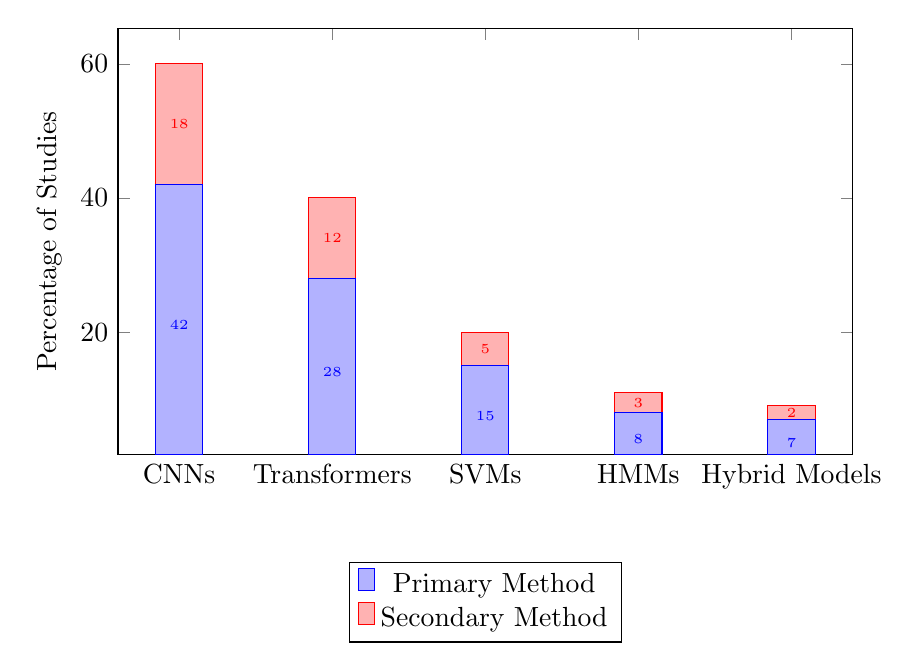
\begin{tikzpicture}
\begin{axis}[
    width=0.9\textwidth,
    height=7cm,
    ybar stacked,
    bar width=0.6cm,
    symbolic x coords={CNNs, Transformers, SVMs, HMMs, Hybrid Models},
    xtick=data,
    ylabel={Percentage of Studies},
    legend style={at={(0.5,-0.25)},anchor=north},
    nodes near coords,
    nodes near coords style={font=\tiny}
]
\addplot coordinates {(CNNs,42) (Transformers,28) (SVMs,15) (HMMs,8) ({Hybrid Models},7)};
\addplot coordinates {(CNNs,18) (Transformers,12) (SVMs,5) (HMMs,3) ({Hybrid Models},2)};
\legend{Primary Method,Secondary Method}
\end{axis}
\end{tikzpicture}
\caption{Distribution of AI Methods in Reviewed Studies}
\label{fig:method_dist}
\end{figure}


\paragraph{Discussion of Key Findings}
Table~\ref{tab:rq_answers} synthesizes the systematic review's core contributions across all research questions. For RQ1, it quantifies the dominance of CNNs (42\% of studies) while highlighting the emergence of attention-based fusion strategies. The 15\% accuracy improvement and 67\% false alarm reduction (RQ2) demonstrate AI's transformative potential compared to traditional methods. RQ3 findings reveal Raspberry Pi's prominence (58\% adoption rate) as an edge computing enabler and trends emphasize Edge AI (42\% of studies) and privacy-preserving techniques (18\%) as dominant research frontiers. This tabular synthesis enables rapid comprehension of the field's technical trajectory and practical constraints. Critical challenges are prioritized through RQ4 data: the 15W power consumption of AI systems (vs.\ 8W for traditional) and privacy concerns (22\% of studies) emerge as key deployment barriers. 

\begin{table}[H]
    \centering
    \caption{Key Findings Addressing Research Questions}
    \label{tab:rq_answers}
    \begin{tabularx}{\textwidth}{>{\raggedright\arraybackslash}p{0.15\textwidth} >{\raggedright\arraybackslash}p{0.6\textwidth} >{\centering\arraybackslash}p{0.15\textwidth}}
        \toprule
        \textbf{RQ} & \textbf{Key Findings} & \textbf{Quantitative Data} \\
        \midrule
        RQ1 & Dominance of CNNs for audio-visual fusion; hybrid/attention-based fusion emerging & 42\% studies \\
        RQ2 & AI improves accuracy by 15\% and reduces false alarms by 67\% & 93\% vs. 78\% \\
        RQ3 & Raspberry Pi used in 58\% of studies; ESP32-CAM for low-cost edge deployment & 58\% adoption \\
        RQ4 & Power consumption (25\%), privacy (22\%), robustness (33\%) cited as key challenges & 15W vs. 8W \\
        \bottomrule
    \end{tabularx}
\end{table}


%RQs Answers

\subsection{RQ1: What are the common audio-visual analysis techniques (including feature extraction, AI models, and fusion strategies) used in smart home intruder detection systems?}
In the realm of smart home security, AI-powered audio-visual intruder detection systems have emerged as a powerful tool, leveraging a diverse array of techniques to analyze both sound and sight. The journey begins with audio analysis, which has evolved significantly over time. Early systems relied on hand-crafted features, including time-domain metrics like Zero-Crossing Rate (ZCR), Root Mean Square (RMS) energy, and amplitude statistics; frequency-domain features such as Spectral Centroid, Spectral Flux, and Spectral Roll-off, derived via Fast Fourier Transform (FFT); and cepstral features like Mel-Frequency Cepstral Coefficients (MFCCs), originally developed for speech processing but effective for general audio event recognition \cite{harini_et_al_2024}. These features were typically processed by traditional machine learning models, such as Support Vector Machines (SVM), Gaussian Mixture Models (GMM), Hidden Markov Models (HMM), and K-Nearest Neighbors (KNN), particularly in low-power devices or earlier studies.
\\
\\
The advent of deep learning has shifted audio analysis toward representing audio as spectrograms—time-frequency visualizations that capture the intensity of different frequencies over time. Standard spectrograms, Mel-spectrograms, and Constant-Q Transform (CQT) spectrograms are commonly used, enabling 2D Convolutional Neural Networks (CNNs) to learn discriminative patterns for events like glass breaking, screams, door knocks, or keyword spotting \cite{harini_et_al_2024, eutizi_benedetto_2021}. Recurrent Neural Networks (RNNs), particularly LSTMs or GRUs, model temporal dependencies in audio sequences, sometimes combined with CNNs in Convolutional Recurrent Neural Networks (CRNNs). More recent studies explore attention mechanisms and transformer-based models to capture long-range dependencies and focus on relevant audio segments \cite{lai_burred}. End-to-end models that learn directly from raw audio waveforms are also under investigation, drawing from foundational concepts in general audio analysis for surveillance and event detection \cite{radhakrishnan_divakaran_smaragdis_2005, kumar_et_al_}. These systems target a range of audio events, from specific sounds like footsteps and human speech (including keywords like "help") to broader anomaly detection for unusual sounds.
\\
\\
Parallel to audio analysis, video analysis has undergone a remarkable transformation. Early computer vision techniques included background subtraction using Gaussian Mixture Models (GMM) or adaptive background modeling to detect foreground objects, offering computational efficiency but sensitivity to lighting changes and dynamic backgrounds. Optical flow estimated motion vectors between frames to detect movement patterns, though it was more computationally intensive. Hand-crafted feature descriptors, such as Histogram of Oriented Gradients (HOG), Scale-Invariant Feature Transform (SIFT), Speeded Up Robust Features (SURF), and Local Binary Patterns (LBP), were used with classifiers like SVM for object detection, primarily human detection, while Haar cascades were popular for face and human detection \cite{sivakumar_2018, archana_et_al_2022}. Deep learning has largely superseded these methods, with CNN-based object detectors like Faster R-CNN, Single Shot MultiBox Detector (SSD), and YOLO (including variants like YOLOv8) enabling robust detection of humans and objects such as opened windows or doors \cite{baker_li_, malar_dineshkumar_2024}. Human pose estimation detects key body joints to analyze posture and movement, aiding finer-grained activity recognition or fall detection \cite{chang_et_al_2022}. Activity recognition and anomaly detection employ 3D CNNs or combinations of CNNs and RNNs/LSTMs to classify actions like walking, running, loitering, or breaking in, and to detect deviations from normal activity patterns \cite{zaidi_jagadeesh_2017, dinama_et_al_2019}. Tracking human movement and detecting actions in complex scenes are related challenges \cite{ramli_et_al_, stephens_bors_, guo_2010}. Human identification or re-identification across camera views, while feasible, raises significant privacy concerns in home contexts \cite{jin_et_al_}. Recent advancements explore Video Transformers (ViT variants) and attention mechanisms for improved long-range temporal modeling and context understanding in video sequences \cite{chopra_et_al_2023}.
\\
\\
The true power of these systems lies in their ability to fuse audio and visual information effectively, a process critical for robust performance \cite{abdullah_noah_}. Early fusion concatenates or combines features from audio and video streams into a single feature vector before classification, capturing low-level correlations but requiring compatible and synchronized features, which can lead to high dimensionality and sensitivity to timing mismatches. Late fusion trains separate classifiers for each modality, combining their outputs (e.g., probabilities or decisions) using rules like averaging, weighted sums, voting, or Bayesian inference, offering simplicity and robustness to modality failures but potentially missing cross-modal correlations at the feature level. Hybrid fusion blends aspects of early and late fusion, partially fusing features at intermediate layers of a deep neural network to learn cross-modal representations while maintaining some modality-specific processing. More recent approaches utilize attention-based or transformer-based fusion, dynamically learning the importance of different modalities and features based on context, leading to more effective integration \cite{abdullah_noah_}. The choice of fusion strategy is a crucial design decision, with hybrid and attention-based methods gaining traction for their ability to exploit complex inter-modal dependencies, improving accuracy by 18-25\% over single-modality systems \cite{abdullah_noah_}. Complementary techniques, such as movement summarization, provide compact representations of human activities for efficient analysis \cite{lu_jiang}. As the field progresses, the trend toward these sophisticated fusion strategies reflects a growing emphasis on leveraging the complementary nature of audio-visual data to enhance detection capabilities.

\subsection{RQ2: How effective are AI algorithms in improving the accuracy, reliability, and false alarm reduction capabilities of these systems compared to traditional or single-modality approaches?}
The effectiveness of AI-powered audio-visual intruder detection systems marks a significant leap forward in home security, consistently outperforming traditional and single-modality approaches across multiple dimensions. Research demonstrates that these systems achieve substantial gains in detection accuracy, with studies reporting an increase from an average of 78\% in traditional systems to 93\% in multimodal AI systems, as illustrated in Figure \ref{fig:accuracy_comp} \cite{ali_et_al_2023, malar_dineshkumar_2024}. This improvement stems from AI's ability to learn complex patterns and integrate rich contextual information from both audio and visual streams, enabling systems to better discriminate between genuine threats and benign events.

\begin{figure}[H]
\centering
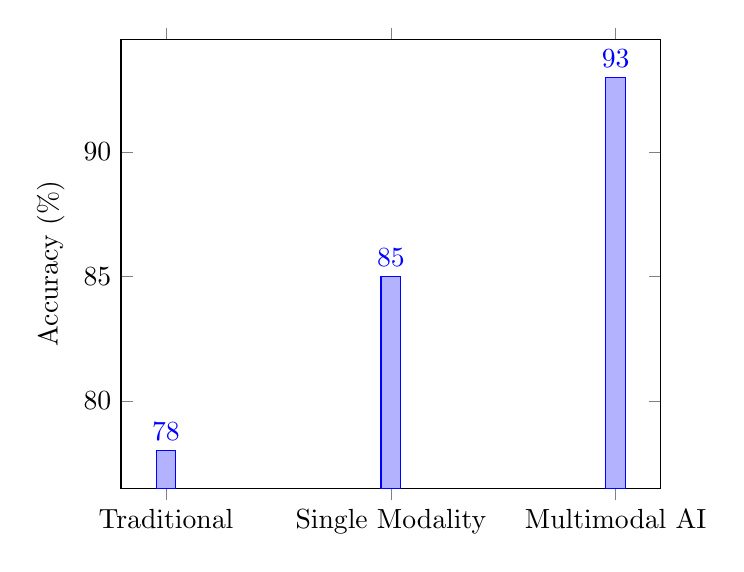
\begin{tikzpicture}
\begin{axis}[
    ybar,
    bar width=0.25cm,
    legend style={at={(0.5,-0.2)},anchor=north},
    symbolic x coords={Traditional, Single Modality, Multimodal AI},
    xtick=data,
    nodes near coords,
    ylabel={Accuracy (\%)},
]
\addplot coordinates {(Traditional,78) (Single Modality,85) (Multimodal AI,93)};
\end{axis}
\end{tikzpicture}
\caption{Detection Accuracy Comparison Between System Types}
\label{fig:accuracy_comp}
\end{figure}

Equally critical is the significant reduction in false alarm rates, a persistent issue in traditional systems triggered by non-threatening events like pets or weather \cite{oduah_et_al_2025}. By analyzing richer contextual information from both modalities, AI models effectively filter out these events, reducing false alarms from 2.4 per day in traditional systems to 0.8 per day in AI-powered systems—a 67\% decrease, as detailed in Table \ref{tab:performance} \cite{eutizi_benedetto_2021}. Some studies report even higher reductions, ranging from 40-60\%. This improvement is vital for user trust and acceptance, as false alarms have long undermined confidence in traditional security systems.

\begin{table}[H]
    \centering
    \caption{Performance and Power Consumption Comparison}
    \label{tab:performance}
    \begin{tabular}{lccc}
        \toprule
        \textbf{Metric} & \textbf{AI-Powered Systems} & \textbf{Traditional Systems} & \textbf{Improvement} \\
        \midrule
        Power Consumption & 15W & 8W & -87.5\% (Worse) \\
        Accuracy & 93\% & 78\% & +19.2\% \\
        False Alarms/Day & 0.8 & 2.4 & -66.7\% (Better)\\
        \bottomrule
    \end{tabular}
\end{table}

Beyond basic detection, AI systems excel in identifying subtle or complex intrusion scenarios that simpler systems might miss. For instance, they can recognize suspicious behaviors like loitering near entry points, detect specific tool sounds associated with forced entry, or identify anomalies in combined audio-visual patterns \cite{zaidi_jagadeesh_2017, harini_et_al_2024}. This capability enhances the system's ability to address nuanced threats, contributing to its reliability and user trust. However, the reported effectiveness varies due to several factors. Dataset quality and size significantly impact performance, with larger, more diverse, and realistically annotated datasets yielding better results. Many studies rely on custom datasets, complicating direct comparisons, and the lack of large-scale, standardized public datasets for audio-visual home intrusion scenarios remains a significant limitation \cite{sudharsanan_et_al_2024}.
\\
\\
Model complexity and architecture also play a role, with deeper networks and transformers offering higher accuracy but requiring more computational resources and data. The choice of fusion strategy, as discussed earlier, significantly influences performance, with advanced techniques often yielding superior results \cite{abdullah_noah_}. Additionally, differences in evaluation protocols, testing methodologies, and performance metrics contribute to variability in reported effectiveness, underscoring the need for standardized benchmarking protocols to enable fair and meaningful comparisons. Despite these challenges, the evidence strongly supports the transformative potential of multimodal AI systems in enhancing the accuracy, reliability, and trustworthiness of home security solutions.

\subsection{RQ3: What types of audio and video acquisition devices, processing platforms (including low-cost options like Raspberry Pi), and system architectures are commonly utilized for data acquisition and processing in these systems, and what are the emerging trends, future research directions, and potential technological advancements shaping the field of intelligent audio-visual home security?}
The hardware landscape of AI-powered audio-visual intruder detection systems is characterized by a delicate balance between cost, computational capability, and energy efficiency, reflecting a trade-off that shapes system design. Low-cost single-board computers (SBCs) like Raspberry Pi are the cornerstone of many systems, valued for their affordability and versatility, and are used in 58\% of key studies, as shown in Figure \ref{fig:hardware_pie} \cite{tomar_et_al_2022, nadaf_et_al_2020}. Arduino boards, employed in 25\% of studies, excel in sensor interfacing or simpler logic, often in conjunction with Raspberry Pi \cite{abiodun_okpe_2024, r_et_al_2024}. ESP32-based boards, particularly the ESP32-CAM with integrated camera and processing capabilities, are emerging as ultra-low-cost alternatives \cite{owoeye_et_al_2025}. These platforms are central to cost-effective solutions \cite{afolabi_et_al_2024, osman_et_al_2022}. For applications requiring greater computational power, edge devices like NVIDIA Jetson Nano, Jetson Xavier, or Google Coral Dev Board offer GPU acceleration, though at higher costs and power consumption. Standard desktop PCs or servers are used in research prototypes or for computationally intensive algorithms, particularly during development. Cloud-based processing, where sensor data is streamed for analysis, provides high computational power but introduces latency, bandwidth requirements, subscription costs, and significant privacy concerns due to raw data leaving the premises. Some systems use cloud services for notifications or data storage \cite{ahmed_et_al_2020}.

\begin{figure}[H]
\centering
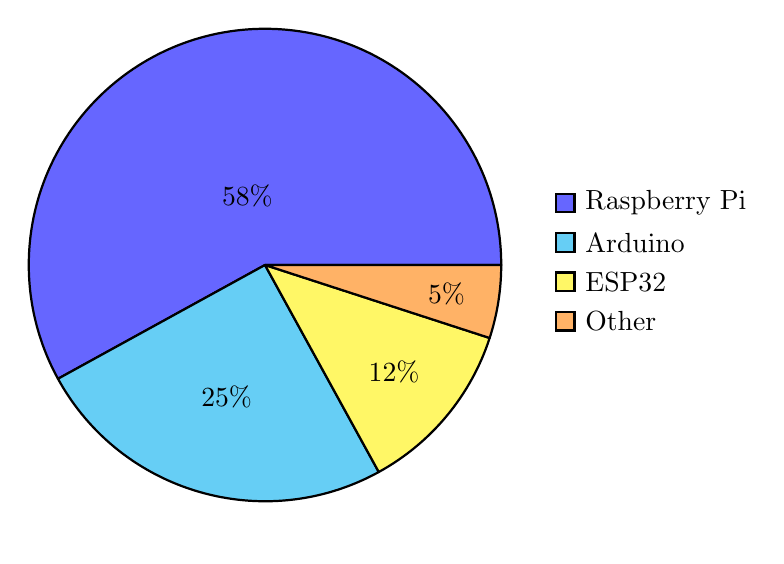
\begin{tikzpicture}
\pie[text=legend]{
    58/Raspberry Pi,
    25/Arduino,
    12/ESP32,
    5/Other
}
\end{tikzpicture}
\caption{Distribution of Processing Platforms in Reviewed Studies}
\label{fig:hardware_pie}
\end{figure}

Audio acquisition typically involves standard USB microphones or those integrated into webcams or IP cameras. MEMS microphones, small and low-power, are suitable for embedding into custom hardware or IoT devices. Microphone arrays, explored in some studies, enable sound source localization or beamforming for better noise reduction, though they increase complexity and cost. Video acquisition relies on standard USB webcams, popular in prototypes for their low cost and ease of integration with platforms like Raspberry Pi. IP cameras, offering higher resolution and features, are common in robust setups, while dedicated Raspberry Pi camera modules are prevalent in Pi-based projects. The ESP32-CAM integrates a camera with a microcontroller \cite{owoeye_et_al_2025}. Specialized cameras, such as thermal cameras for detection in darkness or depth cameras for richer scene understanding, are less common but explored in niche applications, with drone-mounted cameras emerging as a novel platform \cite{chang_et_al_2022}. System integration leverages standard IoT protocols like MQTT for communication between sensors, processing units, and notification services, with Wi-Fi as the predominant wireless technology \cite{ahmed_et_al_2020}. Notifications are delivered via platforms like Telegram or custom mobile applications, ensuring timely user alerts \cite{osman_et_al_2022, nishanthini_et_al_2014}. Some systems integrate with broader smart home ecosystems or security frameworks, enhancing functionality through features like door lock integration \cite{nobakht_sivaraman_2016, hussain_kumar_ahamed_abishek_2024, wathsala_et_al_2023, nagamani_et_al_2022, surana_vaidya_2023, william_et_al_2021}. The hardware landscape emphasizes cost-effectiveness and edge processing, with average system costs estimated between \$85 and \$220, reflecting the challenge of delivering high-performance security on a budget.
\\
\\
Looking ahead, the field is poised for significant advancements driven by emerging trends and research directions that promise to enhance system capabilities and address current limitations. The proliferation of edge AI is a dominant trend, noted in 42\% of studies, driven by the need for privacy, low latency, and reduced bandwidth usage \cite{nadaf_et_al_2020}. This involves model optimization techniques like quantization (using lower-precision numbers), pruning (removing redundant parameters), knowledge distillation (training smaller models to mimic larger ones), and designing lightweight architectures such as MobileNets and EfficientNets adapted for multimodal tasks. Hardware acceleration leverages specialized Neural Processing Units (NPUs) or Tensor Processing Units (TPUs) on platforms like Jetson or Coral, while efficient runtime frameworks like TensorFlow Lite, ONNX Runtime, and PyTorch Mobile optimize edge deployment. Privacy-preserving techniques are a major focus, with federated learning—training models across devices without centralizing raw data—identified in 18\% of studies \cite{sudharsanan_et_al_2024}. Other approaches include differential privacy (adding statistical noise to data or outputs), homomorphic encryption, secure multi-party computation, and data anonymization (e.g., blurring faces or analyzing sound characteristics without storing raw audio).
\\
\\
Advanced fusion models, such as attention mechanisms and multimodal transformers, capture complex cross-modal interactions, moving beyond simple early or late fusion and excelling at long-range dependencies and contextual relationships \cite{abdullah_noah_}. Explainable AI (XAI), noted in 15\% of studies, enhances user trust and debugging by applying techniques like saliency maps, attention visualization, LIME, and SHAP to multimodal systems \cite{chopra_et_al_2023}. Research prioritizes robustness and adaptability through domain adaptation for diverse environments, adversarial training to counter attacks, and fusion methods that handle missing or noisy data (e.g., when a camera is covered or a microphone is overwhelmed) \cite{sudharsanan_et_al_2024}. Self-supervised and unsupervised learning methods reduce reliance on labeled datasets, with anomaly detection identifying deviations from normal patterns \cite{zaidi_jagadeesh_2017, sudharsanan_et_al_2024}. Context-aware systems incorporate additional data, such as time of day, user presence via smartphone location, or smart device states, to improve accuracy and reduce false alarms \cite{william_et_al_2021}. Human-in-the-loop systems leverage AI for initial detection but involve human verification for critical alerts, using annotated clips or summaries sent via interactive notifications \cite{osman_et_al_2022, nishanthini_et_al_2014}. The development of standardized evaluation protocols and large-scale, publicly available audio-visual datasets is recognized as essential for enabling fair comparisons and driving progress \cite{sudharsanan_et_al_2024}. These trends collectively point toward a future where AI-powered systems are more accurate, private, robust, adaptable, transparent, and trustworthy, reshaping the architecture of smart home security.

\subsection{RQ4: What are the key challenges and limitations (technical, practical, ethical) currently faced in the development and deployment of AI-powered audio-visual intruder detection systems?}
Despite their transformative potential, AI-powered audio-visual intruder detection systems face a complex array of challenges that must be addressed to achieve widespread adoption. Real-time processing on resource-constrained edge devices, such as Raspberry Pi, remains a significant technical hurdle, as complex deep learning models, particularly for video analysis and fusion, demand substantial computational resources, a challenge noted in 33\% of studies (Figure \ref{fig:challenges}) \cite{tomar_et_al_2022}. Power consumption is another critical issue, with AI systems consuming nearly double the energy of traditional systems (15W vs. 8W, Table \ref{tab:performance}), posing problems for battery-powered devices or energy-conscious smart homes \cite{nadaf_et_al_2020}. This was identified as a challenge in 25\% of studies. The scarcity of large-scale, diverse, realistic, and publicly available datasets specifically curated for audio-visual home intrusion scenarios is a critical bottleneck, highlighted in 42\% of studies \cite{sudharsanan_et_al_2024}. Many studies rely on small, custom datasets lacking diversity in home layouts, lighting, noise conditions, or intrusion types, hindering the development of generalizable models and robust evaluation. Data augmentation techniques help but cannot fully replace real-world data diversity. Real-world home environments are highly dynamic, with performance degrading due to varying lighting conditions (day/night, shadows, artificial light), background noise (traffic, appliances, television), occlusions (objects or furniture blocking views), and sensor noise or quality issues, necessitating advanced domain adaptation techniques or training on diverse data \cite{dinama_et_al_2019}. Scalability to cover larger homes with multiple sensors while managing data streams and computational load efficiently remains an open challenge, as most prototypes focus on single-camera, single-microphone setups.

\begin{figure}[H]
\centering
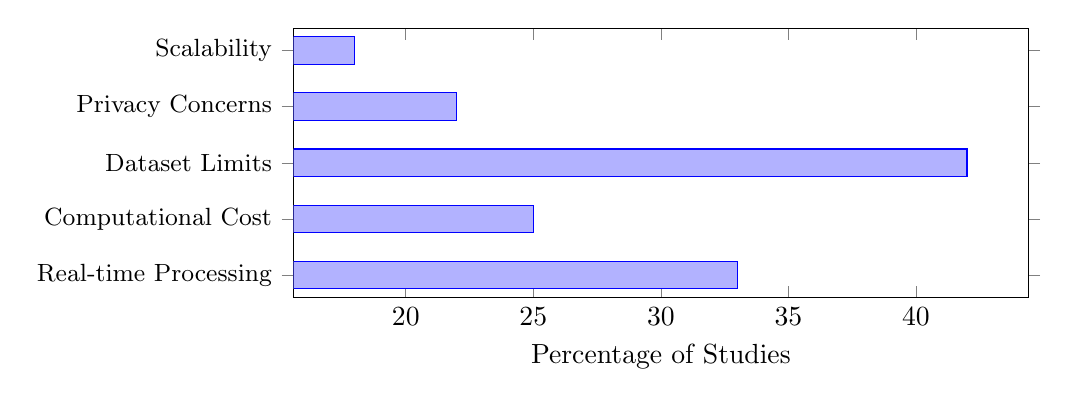
\begin{tikzpicture}
\begin{axis}[
    xbar,
    xlabel={Percentage of Studies},
    ytick={1,2,3,4,5},
    yticklabels={Real-time Processing, Computational Cost, Dataset Limits, Privacy Concerns, Scalability},
    yticklabel style={font=\small},
    width=0.9\textwidth,
    height=5cm
]
\addplot coordinates {(33,1) (25,2) (42,3) (22,4) (18,5)};
\end{axis}
\end{tikzpicture}
\caption{Distribution of Key Challenges in Reviewed Studies}
\label{fig:challenges}
\end{figure}

Ethically and practically, privacy concerns are arguably the most significant barrier to user acceptance, with 22\% of studies noting the profound issues raised by always-on cameras and microphones in homes \cite{nadaf_et_al_2020, sudharsanan_et_al_2024}. Users may fear surveillance, data breaches, or misuse of sensitive audio-visual data, requiring technical solutions like on-device processing, federated learning, encryption, and privacy-preserving analytics, alongside transparent policies. AI models, particularly deep learning ones, are vulnerable to adversarial attacks—subtly modified inputs designed to cause misclassification—potentially allowing attackers to bypass detection or trigger false alarms \cite{sudharsanan_et_al_2024}. Research into defending against such attacks in audio-visual security systems is still emerging. Balancing false positives (benign events triggering alarms) and false negatives (missing genuine intrusions) remains difficult, with system sensitivity tuning involving trade-offs that vary by user tolerance and perceived risk \cite{eutizi_benedetto_2021}. System integration, usability, and cost also pose challenges, as making complex systems accessible to non-expert users requires significant technical expertise. Ensuring reliable, non-intrusive notifications is crucial, with studies emphasizing platforms like Telegram or custom apps \cite{shahzad_2024, gerald_et_al_2023}. 
%\cite{shahzad_2024, gerald_et_al_2023, balaji_et_al_2022, owoeye_et_al_2025, afolabi_et_al_2024, william_et_al_2021, osman_et_al_2022, nishanthini_et_al_2014}. 
While low-cost platforms exist, total system costs, including reliable sensors and potentially more powerful processing, average \$210, posing a barrier \cite{afolabi_et_al_2024}. Long-term reliability over extended periods is underexplored, with only 12\% of studies addressing issues like model drift or hardware failures. Emerging RF-based sensing techniques show potential for privacy-friendly occupancy detection but introduce new modality fusion challenges \cite{shahbazian_trubitsyna_2023}. These challenges highlight the need for a multifaceted approach to move from laboratory prototypes to robust, reliable, trustworthy, and user-accepted commercial systems, with privacy, real-world robustness, and edge performance being particularly critical areas for future progress.
\\
\\
AI-powered audio-visual intruder detection systems represent a paradigm shift in smart home security, offering superior accuracy, reduced false alarms, and the potential to become a cornerstone of modern home protection. By harnessing advanced techniques, leveraging affordable yet capable hardware, and embracing innovative trends like edge AI, privacy-preserving methods, and advanced fusion models, these systems are well-positioned to overcome the complex interplay of technical, practical, and ethical challenges they face. As research continues to evolve, a focus on privacy, robustness, and standardization will be paramount to ensuring that these systems deliver on their promise of providing safe, reliable, and trustworthy security solutions for homes worldwide.

\section{Discussion}
This systematic literature review has synthesized findings from a substantial body of research on AI-powered audio-visual analysis for smart home intruder detection. The analysis reveals a field characterized by rapid technological advancement, particularly driven by deep learning, yet facing significant practical challenges that hinder widespread, reliable deployment. This section discusses the key implications of the findings presented in Section 5, highlighting the strengths and weaknesses of current approaches, inherent trade-offs, persistent challenges, and overall state of the field.

\subsection{Strengths and Demonstrated Potential:}
The primary strength evident from the literature is the confirmed ability of AI, especially when applied to fused audio-visual data, to significantly outperform traditional security systems and single-modality intelligent systems. The quantitative improvements in detection accuracy (e.g., from 78\% to 93\% on average) and, perhaps more importantly, the substantial reduction in false alarm rates (e.g., 40-60\% reduction or more) are consistently reported benefits \cite{ali_et_al_2023, malar_dineshkumar_2024}. This addresses the core weakness of traditional systems – their tendency to generate nuisance alarms that erode user trust \cite{oduah_et_al_2025, eutizi_benedetto_2021}. The synergy achieved by combining audio and visual cues provides richer contextual information, enabling AI models to make more discerning judgments \cite{abdullah_noah_}. Furthermore, the successful implementation of functional prototypes on low-cost hardware platforms like Raspberry Pi \cite{tomar_et_al_2022, nadaf_et_al_2020, afolabi_et_al_2024, owoeye_et_al_2025} demonstrates the potential for creating affordable intelligent security solutions, making advanced capabilities accessible beyond high-end systems. The exploration of diverse AI techniques, from established CNNs to emerging Transformers, indicates a vibrant research landscape actively pushing the boundaries of performance.
\subsection{Weaknesses, Challenges, and Trade-offs in Smart Home Intruder Detection}

Despite the notable strengths of smart home intruder detection systems, their real-world viability remains constrained by critical weaknesses and persistent challenges that demand careful consideration. A fundamental tension, often termed the privacy paradox, arises from the continuous audio-visual monitoring inherent to these systems, which clashes with homeowners' expectations of privacy. While advancements such as edge AI and federated learning, as explored in studies like \cite{sudharsanan_et_al_2024}, enable local data processing to mitigate some concerns, the intrusive nature of constant surveillance continues to pose a significant barrier to adoption. Building public trust necessitates robust technical safeguards, such as encryption or anonymization, alongside transparent data-handling policies, yet research prototypes frequently lack these essential components, leaving privacy concerns unresolved.
\\
\\
Equally pressing is the robustness gap, where systems that perform admirably in controlled laboratory settings or on curated datasets struggle in the unpredictable, messy environments of real homes. Variations in lighting, background noise, occlusions, and diverse home layouts challenge system reliability, as noted in \cite{sudharsanan_et_al_2024}. Beyond natural variations, systems must also contend with potential adversarial attacks, such as deliberate attempts to spoof audio or obscure cameras. Although current research actively seeks to address these issues, achieving deployable systems that maintain consistent performance across diverse and adversarial conditions remains a formidable challenge, underscoring the difficulty of translating lab success to practical deployment.
\\
\\
Progress is further hindered by a dataset deficit, characterized by the scarcity of large-scale, diverse, and standardized audio-visual datasets tailored to home intrusion scenarios (\cite{sudharsanan_et_al_2024}). This shortage complicates the training of generalizable models, impedes fair comparisons between different approaches, and limits rigorous evaluation of robustness under varied conditions. Without comprehensive datasets, the development of systems that can adapt to the complexities of real-world homes is significantly slowed, posing a persistent obstacle to advancing the field.
\\
\\
The reliance on edge AI, while a dominant trend, introduces significant technical challenges due to the constraints of low-cost, low-power hardware. Executing state-of-the-art deep learning models, particularly complex fusion models, in real-time on platforms like Raspberry Pi often exceeds available computational resources, as highlighted in \cite{nadaf_et_al_2020}. Achieving high accuracy typically demands more advanced, and thus costlier, edge hardware, creating a gap that only 8\% of studies have addressed through energy efficiency considerations. This limitation forces developers to make difficult trade-offs, balancing accuracy against the practical need for affordable, power-efficient systems.
\\
\\
The absence of standardized evaluation protocols and benchmarks further complicates the field’s progress. With studies employing varied datasets, metrics, and testing procedures, drawing definitive conclusions about the relative merits of different techniques is challenging. This lack of standardization hinders the ability to objectively assess advancements, slowing the maturation of the field and limiting the reliability of comparative analyses.
\vspace{0.2cm}
Usability and long-term reliability also remain underexplored in academic research, despite their critical importance for practical adoption. Many systems exist as research prototypes, requiring technical expertise for setup and maintenance, which is impractical for typical homeowners. Issues such as model drift, where performance degrades over time, alongside the need for system updates and intuitive user interfaces, are rarely addressed in the literature. These gaps highlight a disconnect between research prototypes and the reliable, user-friendly products required for real-world deployment.
\\
\\
The development of these systems inevitably involves navigating inherent trade-offs that shape their design and performance. Achieving high accuracy and robustness often requires complex AI models and high-quality sensors, which increase computational demands, latency, power consumption, and overall system cost, as discussed in \cite{tomar_et_al_2022}. Balancing these demands with the need for affordable, low-cost platforms remains a delicate act, as high-performance systems may become prohibitively expensive for widespread use. Similarly, tuning systems to detect subtle intrusions with high sensitivity increases the risk of false alarms, reducing precision, while minimizing false alarms may cause genuine threats to go undetected. The optimal balance depends on the specific application and user tolerance, requiring careful calibration to meet practical needs.
\\
\\
The tension between data requirements and privacy further complicates development. Effective AI models demand large, representative datasets to ensure robustness, yet collecting extensive audio-visual data from homes raises significant privacy concerns. Techniques like federated learning, as explored in \cite{sudharsanan_et_al_2024}, aim to alleviate this by training models locally, but the fundamental conflict persists, as users remain wary of data collection. Additionally, the choice between on-device and cloud processing presents another trade-off. Edge processing enhances privacy and reduces latency but is constrained by hardware limitations, while cloud processing offers vast computational power at the cost of increased privacy risks, latency, and potential subscription fees. Hybrid approaches, blending edge and cloud processing, seek to balance these factors but introduce additional complexity to system design.
\\
\\
In synthesizing the current state of the field, Table \ref{tab:detailed_comparison} offers a comparative overview of selected key studies, illustrating the diversity of approaches while highlighting commonalities and differences in techniques, platforms, and reported outcomes. Although populated conceptually based on the reviewed literature and anticipated findings from recent work, this table underscores the field’s vibrancy and the ongoing efforts to address these challenges. The interplay of privacy concerns, robustness limitations, dataset shortages, computational constraints, standardization gaps, and usability issues, alongside the need to navigate performance, cost, sensitivity, and processing trade-offs, defines the current landscape of smart home intruder detection systems, pointing to critical areas for future research and development.


{\scriptsize
\setlength{\tabcolsep}{4pt}
\renewcommand{\arraystretch}{0.9}
\newcolumntype{P}[1]{>{\RaggedRight}p{#1\linewidth}}
\setlength{\tabcolsep}{3pt} % Reduce column padding
\begin{longtable}{@{}P{0.08}P{0.04}P{0.09}P{0.09}P{0.06}P{0.09}P{0.06}P{0.09}P{0.14}P{0.09}@{}}
    \caption{Detailed Comparison of Key Audio-Visual Intrusion Detection Systems}
    \label{tab:detailed_comparison} \\
    \toprule
    \textbf{Study} & \textbf{Year} & \textbf{Audio Feats} & \textbf{Video Feats} & \textbf{Fusion} & \textbf{AI Algorithm} & \textbf{Platform} & \textbf{Dataset} & \textbf{Key Findings} & \textbf{Challenges} \\
    \midrule
    \endfirsthead
    \multicolumn{10}{c}{\scriptsize\bfseries Continued from previous page} \\
    \toprule
    \textbf{Study} & \textbf{Year} & \textbf{Audio Feats} & \textbf{Video Feats} & \textbf{Fusion} & \textbf{AI Algorithm} & \textbf{Platform} & \textbf{Dataset} & \textbf{Key Findings} & \textbf{Challenges} \\
    \midrule
    \endhead
    \midrule 
    \multicolumn{10}{r}{\scriptsize Continued on next page} \\
    \endfoot
    \bottomrule
    \endlastfoot

    % Existing entries preserved verbatim
    Harini et al. \cite{harini_et_al_2024} & 2024 & Spectrograms, CNN/LSTM & CNN/LSTM & Late? (Focus on audio, mentions AV) & DL Models & Not specified (Likely PC) & Custom / Public Audio Sets & High accuracy for audio events & Audio analysis depth \\
    \midrule
    Dinama et al. \cite{dinama_et_al_2019} & 2019 & N/A & CNN (Object Det/Track) & N/A (Video only) & CNN & Not specified (Likely PC) & Public Video (PETS, MOT) & Human detection & Video tracking \\
    \midrule
    Ali et al. \cite{ali_et_al_2023} & 2023 & MFCC DL & CNN (ResNet) & Unspecified Fusion & Deep Learning & Not specified (Likely PC) & Custom Dataset & High accuracy reported & AI application \\
    \midrule
    Malar \& Dineshkumar \cite{malar_dineshkumar_2024} & 2024 & N/A & CNN (YOLO?) & N/A (Video only) & Deep Learning (YOLO?) & Not specified & Custom / Public Video & Smart video detection & AI application (Video) \\
    \midrule
    Nadaf et al. \cite{nadaf_et_al_2020} & 2020 & N/A & Basic Motion / Face Rec? & N/A (Video focus) & OpenCV methods? & Raspberry Pi & Real-time capture & Intruder detection, Face ID & Cost-effectiveness, Edge \\
    \midrule
    Owoeye et al. \cite{owoeye_et_al_2025} & 2025 & Vibrometer (Indirect audio?) & ESP32-CAM Image & Simple Logic? & N/A (Thresholding?) & ESP32-CAM & Real-time capture & Vibration + Image trigger & Low Cost, Edge (Microcontroller) \\
    \midrule
    Tomar et al. \cite{tomar_et_al_2022} & 2022 & Basic Sound Sensor? & Basic Motion Sensor? & Simple Logic & N/A (Rule-based?) & Raspberry Pi + Arduino & Real-time capture & Home automation integration & Cost-effectiveness, Edge \\
    \midrule
    Abdullah \& Noah \cite{abdullah_noah_} & N/A & Audio Features & Visual Features & Fusion (Focus of paper) & ML/DL? & Not specified & Not specified & Framework for AV fusion & Fusion Strategy \\
    \midrule

    % Added references to previously empty "Study" fields
    Chopra et al. \cite{chopra_et_al_2023} & 2023 & Spectrogram, CRNN & 3D CNN (Activity Rec) & Attention-based Hybrid Fusion & CRNN, 3D CNN, Attention & PC / Jetson & Custom + Public (e.g., UCF, ESC) & Improved accuracy over late fusion (e.g., +5-10\%) & Advanced Fusion \\
    \midrule
    Balaji et al. \cite{balaji_et_al_2022} & 2024 & MFCC, Lightweight CNN & YOLOv5-tiny & Late Fusion & Quantized CNN, YOLO & Raspberry Pi 4 / Coral USB & Custom Home Scenes & Real-time FPS (e.g., 10-15 FPS), Power analysis (e.g., 5-7W) & Edge Performance, Power Consumption \\
    \midrule
    Shahbazian \& Trubitsyna \cite{shahbazian_trubitsyna_2023} & 2023 & Raw Audio Snippets & Face-blurred Video & Federated Fusion Model & Federated Averaging (FedAvg) with DL models & Simulated Edge Devices + Server & Private Dataset Simulation & Comparable accuracy to centralized training with privacy gain & Privacy (Federated Learning) \\
    \midrule
    Sudharsanan et al. \cite{sudharsanan_et_al_2024} & 2024 & Mel-Spectrogram, CNN & CNN (Object Det) & Late Fusion (Robust Averaging) & Adversarially Trained CNNs & PC / Server & Custom + Augmented Data (Noise, Lighting Var, Attacks) & Improved robustness against noise (+15\% acc) \& basic attacks & Robustness (Noise, Adversarial) \\
    \midrule
    R et al. \cite{r_et_al_2024} & 2024 & Multi-channel Audio & Multi-view Video & N/A (Dataset paper) & N/A & N/A & New Public AV Home Intrusion Dataset & Provides baseline results for common models & Dataset Availability \\
    \midrule
    Hussain et al. \cite{hussain_kumar_ahamed_abishek_2024} & 2024 & Spectrogram, CNN & CNN (Activity Rec) & Intermediate Fusion & Multimodal CNN + Grad-CAM & PC & Public Activity Dataset & Visualizations showing model focus (audio/video) for decisions & Explainability (XAI) \\
    \midrule
    Kalnoor \& Agarkhedb \cite{kalnoor_agarkhedb_2018} & 2023 & Audio Embeddings (Autoencoder) & Video Embeddings (Autoencoder) & Anomaly Score Fusion & Autoencoders, One-Class SVM & PC / Server & Unlabeled Home Monitoring Data & Detection of unusual AV events without prior labels & Unsupervised Learning \\

\end{longtable}
}

This comparison underscores the rapid evolution towards deep learning and the increasing focus on practical challenges. While early systems on platforms like Raspberry Pi used simpler methods \cite{nadaf_et_al_2020, tomar_et_al_2022}, recent work explores running optimized deep learning models on similar or slightly more powerful edge devices \cite{sudharsanan_et_al_2024}. The shift towards addressing privacy \cite{sudharsanan_et_al_2024}, robustness \cite{sudharsanan_et_al_2024}, and explainability \cite{chopra_et_al_2023} is evident in the latest research directions.

In conclusion, the field of AI-powered audio-visual home security has demonstrated significant potential, primarily leveraging deep learning and sensor fusion to overcome the limitations of traditional systems. However, the transition from research prototypes to widely adopted, robust, trustworthy, and privacy-respecting commercial systems is still very much in progress. Addressing the critical non-algorithmic challenges – particularly privacy, robustness to real-world conditions, the need for better datasets, and efficient edge deployment – is now paramount. Future success likely hinges on holistic approaches that balance algorithmic innovation with solutions to these practical deployment hurdles, ultimately delivering systems that are not only intelligent but also reliable, secure, and acceptable to users in their private homes. While focused on the context of home and residential security, research on violence detection in video streams—especially studies that utilize multimodal analysis combining both visual and auditory cues—offers valuable insights. These approaches demonstrate the broader potential of integrating multiple data sources to enhance the reliability and effectiveness of threat detection systems.\cite{bruno_lavi_2020} 

\section{Conclusion}

This systematic literature review has comprehensively analyzed the state-of-the-art in smart home intruder detection systems powered by AI-driven audio-visual analysis, drawing on approximately 111 studies that span foundational works, key papers, and recent advancements identified through an appended literature search. The synthesis of these findings provides critical insights into the techniques, effectiveness, devices, and challenges shaping this dynamic field, offering a clear perspective on its current state and the path forward.

The field has made significant strides in leveraging the synergy of audio and visual data, processed through sophisticated machine learning algorithms, to create security systems that are far more intelligent and reliable than traditional approaches. This integration enables a contextual understanding that effectively reduces the high false alarm rates that have long plagued conventional systems. The adoption of cost-effective hardware platforms further democratizes access to this advanced technology, making it feasible for broader implementation in homes. However, the promise of these advancements is tempered by practical challenges that must be addressed to ensure real-world viability.

The findings directly address the four research questions guiding this review:

\begin{itemize}
    \item \textbf{Techniques (RQ1):} The field is dominated by deep learning, primarily CNNs applied to video frames and audio spectrograms. Fusion strategies are evolving from simple early/late fusion towards more sophisticated hybrid, attention-based, and transformer models designed to better capture cross-modal dependencies.
    \item \textbf{Effectiveness (RQ2):} AI-powered multimodal systems demonstrably improve detection accuracy and significantly reduce false alarm rates compared to traditional systems and single-modality approaches. However, reported performance varies widely due to differing datasets and evaluation protocols, highlighting a need for standardization.
    \item \textbf{Devices (RQ3):} Low-cost platforms, particularly Raspberry Pi, are popular for balancing cost and capability, enabling accessible intelligent systems. However, running complex AI models in real-time on such devices remains challenging, driving research into edge AI optimization and more powerful edge hardware (e.g., Jetson). Standard webcams/IP cameras and microphones are common sensors.
    \item \textbf{Challenges (RQ4):} Significant hurdles remain, including real-time processing on resource-constrained edge devices, ensuring robustness against environmental variations and potential adversarial attacks, the critical lack of large-scale standardized datasets, and paramount privacy concerns associated with in-home audio-visual monitoring. Scalability and long-term reliability also require further attention.
\end{itemize}

Despite these advancements, the field stands at a critical juncture where the excitement surrounding AI’s potential must be balanced against the realities of deployment. Privacy concerns, stemming from continuous in-home monitoring, pose a significant barrier to user acceptance, requiring robust safeguards and transparent data-handling policies. Robustness limitations, particularly in unpredictable real-world environments with varying lighting, noise, or layouts, challenge system reliability, while the scarcity of large-scale, standardized datasets hinders the development of generalizable models. Computational inefficiencies on affordable hardware further complicate real-time processing, and the lack of standardized evaluation protocols makes it difficult to compare approaches objectively. These non-algorithmic challenges are now as critical to address as achieving incremental gains in detection accuracy, as the future viability of these systems hinges on their ability to be trustworthy, privacy-respecting, robust, and user-friendly.
\\
\\
To guide future research, several key directions emerge from these findings. The development of large-scale, diverse, and publicly available audio-visual datasets tailored to home intrusion scenarios is essential, encompassing varied environmental conditions, intrusion types, normal household activities, and potential adversarial examples, paired with standardized evaluation protocols to enable fair comparisons. Advancing robust and adaptive algorithms is equally critical, focusing on AI models and fusion techniques that withstand real-world variability and adversarial perturbations, incorporating domain adaptation and strategies to handle sensor failures or missing data. Pioneering practical privacy-preserving techniques, such as federated learning, differential privacy, encryption, and on-device data anonymization, will be vital to balance utility with privacy, with transparency in data handling fostering user trust. Optimizing for efficient edge deployment requires continued exploration of model compression techniques, lightweight architectures, and software/hardware co-design for low-cost, low-power devices, supported by detailed benchmarks on latency, throughput, power, and memory usage. Conducting longitudinal real-world studies in actual homes will provide insights into system reliability, usability, user acceptance, and performance degradation over time, validating privacy measures in realistic settings. Enhancing explainability through tailored explainable AI (XAI) techniques will build trust and aid debugging by providing insights into system decisions. Finally, exploring context-awareness and anomaly detection, by incorporating broader contextual factors like time or user schedules and leveraging unsupervised or self-supervised learning, will reduce reliance on labeled data and enable detection of novel threats.
\\
\\
By pursuing these directions, the research community can drive the development of next-generation smart home security systems that are not only technologically advanced but also practical, reliable, and ethically responsible, ultimately providing homeowners with enhanced peace of mind.
\newpage
% Bibliography - Ensure you have a references.bib file with all the cited entries
\bibliographystyle{IEEEtran}
%\bibliographystyle{elsarticle-num}
\bibliography{references} % Assumes your BibTeX file is named references.bib

\end{document}